%% V1.0
%% 2019/01/16
%% This is the template for a Lab report following an IEEE paper. Modified by Francisco Tovar after Michael Sheel original document.

%% This is a skeleton file demonstrating the use of IEEEtran.cls
%% (requires IEEEtran.cls version 1.8b or later) with an IEEE
%% journal paper.
%%
%% Support sites:
%% http://www.michaelshell.org/tex/ieeetran/
%% http://www.ctan.org/pkg/ieeetran
%% and
%% http://www.ieee.org/


\documentclass[journal]{IEEEtran}

% *** CITATION PACKAGES ***
\usepackage[style=ieee]{biblatex} 
\usepackage[spanish]{babel}
\usepackage{amssymb}
\bibliography{references.bib}    %your file created using JabRef

% *** MATH PACKAGES ***
\usepackage{amsmath}
\usepackage{listings}
\usepackage{xcolor}
\lstset{
    backgroundcolor=\color{lightgray},   % Background color for code
    basicstyle=\ttfamily\footnotesize,     % Font style and size
    keywordstyle=\color{blue},             % Color for keywords
    commentstyle=\color{green},            % Color for comments
    stringstyle=\color{red},               % Color for strings
    numbers=left,                          % Line numbers on the left
    numberstyle=\tiny\color{gray},         % Style for line numbers
    stepnumber=1,                          % Show line numbers every 1 line
    numbersep=5pt,                         % Distance between line numbers and code
    showstringspaces=false                 % Don't show spaces in strings
}

% *** PDF, URL AND HYPERLINK PACKAGES ***
\usepackage{url}
% correct bad hyphenation here
\hyphenation{op-tical net-works semi-conduc-tor}
\usepackage{graphicx}  %needed to include png, eps figures
\usepackage{float}  % used to fix location of images i.e.\begin{figure}[H]

\begin{document}

% paper title
\title{Proyecto: Street View House Numbers (SVHN)}

% author names 
\author {Braulio Isaac Martínez Aceves 747200
        }% <-this % stops a space
        
% The report headers
\markboth{MSC1007A Aprendizaje Automático, Reporte de Proyecto SVHN, 16 noviembre 2024}%do not delete next lines
{Shell \MakeLowercase{\textit{et al.}}: Bare Demo of IEEEtran.cls for IEEE Journals}

% make the title area
\maketitle

%\begin{IEEEkeywords}
%keywords, temperature, xxxx equation, etc.
%\end{IEEEkeywords}

\section{Introducción y justificación}
% Here we have the typical use of a "W" for an initial drop letter
% and "RITE" in caps to complete the first word.
% You must have at least 2 lines in the paragraph with the drop letter
% (should never be an issue)

El dataset SVHN representa dígitos en imágenes naturales que provienen de fotografías de casas. Detectar y leer texto en fotografías representa un problema complicado en la disciplina de visión por computadora. Si bien algunos problemas de reconocimiento de caracteres bien delimitados se encuentran resueltos (OCR, reconocimiento de dígitos escritos a mano), el reconocimiento en escenas o imágenes naturales representa un reto mayor debido a los artefactos, ruido o distractores naturales.\cite{svhn} Estas características presentan al dataset como un buen candidato para temas de machine learning.

\section{Objetivos}
\begin{itemize}
        \item Obtención de datos
        \item Preprocesamiento y Feature Engineering
        \item Selección de modelos
        \item Cross-Validation
        \item Entrenamiento y evaluación
\end{itemize}


\subsection{Obtención de datos}
El dataset se obtuvo directamente de HugginFace.\cite{huggingface_svhn}
\begin{lstlisting}[language=Python]
from datasets import load_dataset
ds = load_dataset("ufldl-stanford/svhn",
                  "cropped_digits"
                 )
\end{lstlisting}


\subsection{Preprocesamiento y Feature Engineering}
Debido a la complejidad del problema (dígitos en imágenes naturales a color y con distractores), es de vital importancia realizar el correcto pre-procesamiento y Feature Engineering para facilitar la tarea y rendimiento de nuestro algoritmo predictivo. Como objetivo final se busca reconocer dígitos centrados en imágenes de 32x32, como primera aproximación, se transforma y reduce la imagen a color original a bordes. Para esto, se propone la siguiente lista ordenada de pasos o transformaciones a realizar en cada muestra antes de realizar cualquier entrenamiento:

\begin{enumerate}
        \item Escala de grises: Reducción de 3 canales (RGB) a 1 canal
        \item Sharpening: Mejorar la claridad de la imagen para poder extraer más características
        \item CLAHE: Contrast Limited Adaptive Histogram Equalization, usado para mejorar el contraste de la imagen y reducir ruido
        \item Transformación logarítmica o con mediana: Normalizar los datos para evitar que valores poco comunes (outliers) afecten el entrenamiento
        \item Binary Dynamic Thresholding: Reducir el espacio de escala de grises a [0, 1]
        \item Filtro Gaussiano: Reducir el impacto de posibles distractores laterales a los bordes de la imagen
        \item Flattening: Se convierten las imágenes 2D de 32x32 a un solo vector 1D de 1024 elementos
\end{enumerate}

\subsubsection{Visualización de Transformaciones, dígito 9}
En la siguiente secuencia de imágenes se puede observar, paso a paso, las transformaciones a una muestra.

\begin{figure}[H]
        \centering
        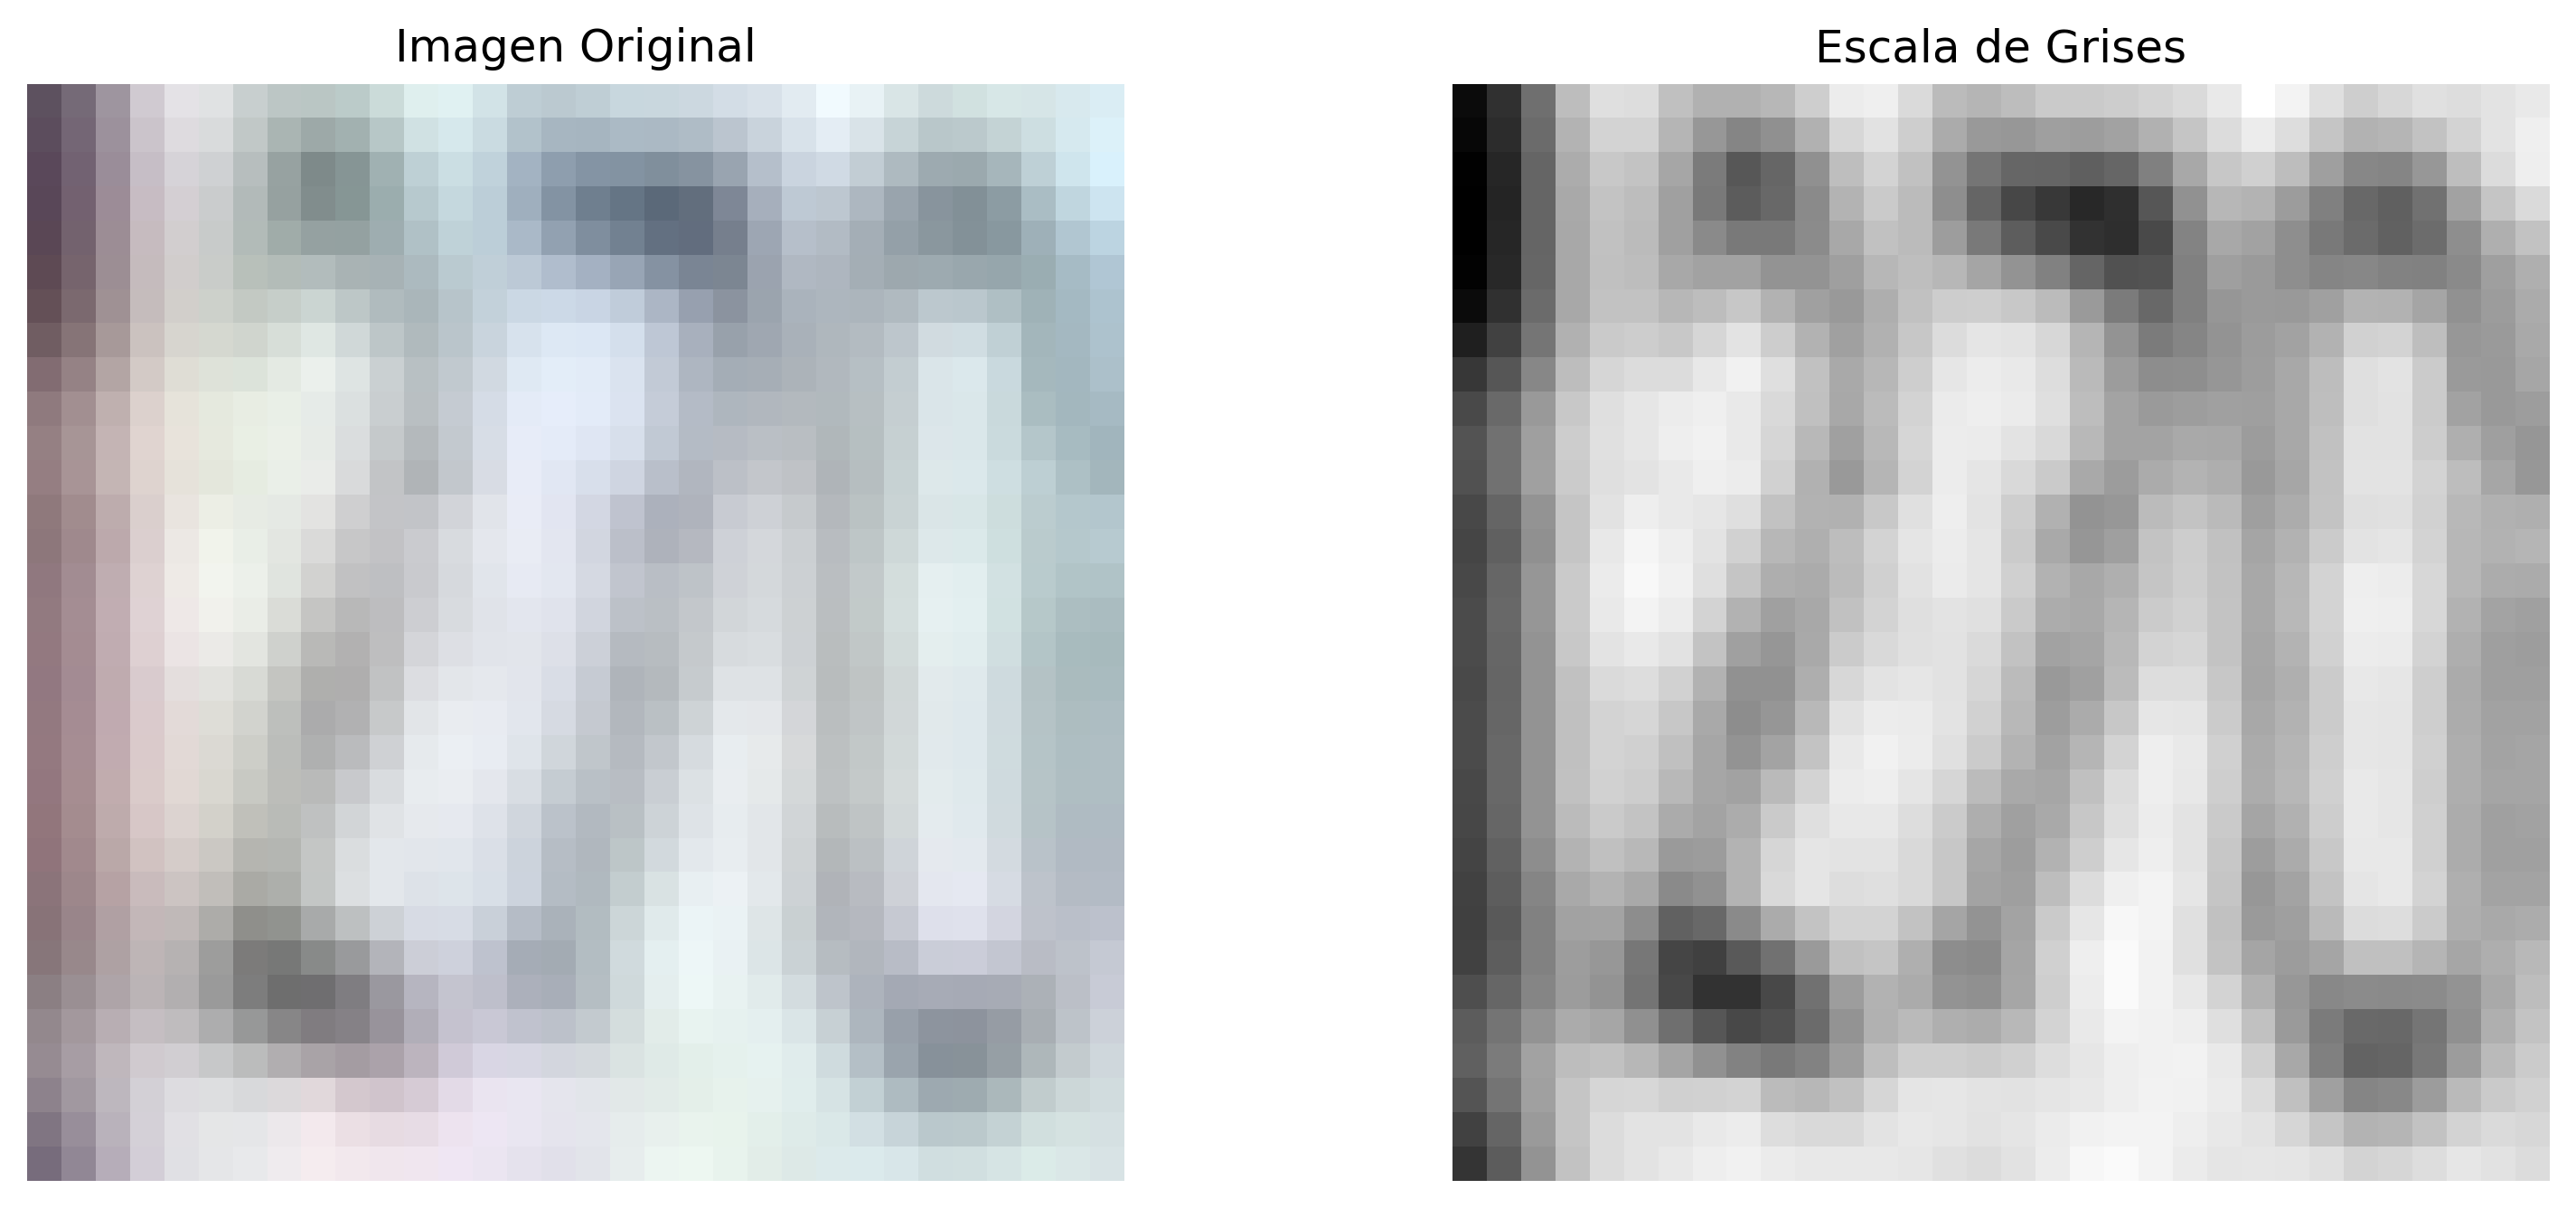
\includegraphics[width=\linewidth]{figures/row_1_images.png}
        \caption{Imagen original y transformación a escala de grises}
        \label{fig:row_1}
\end{figure}

\begin{figure}[H]
        \centering
        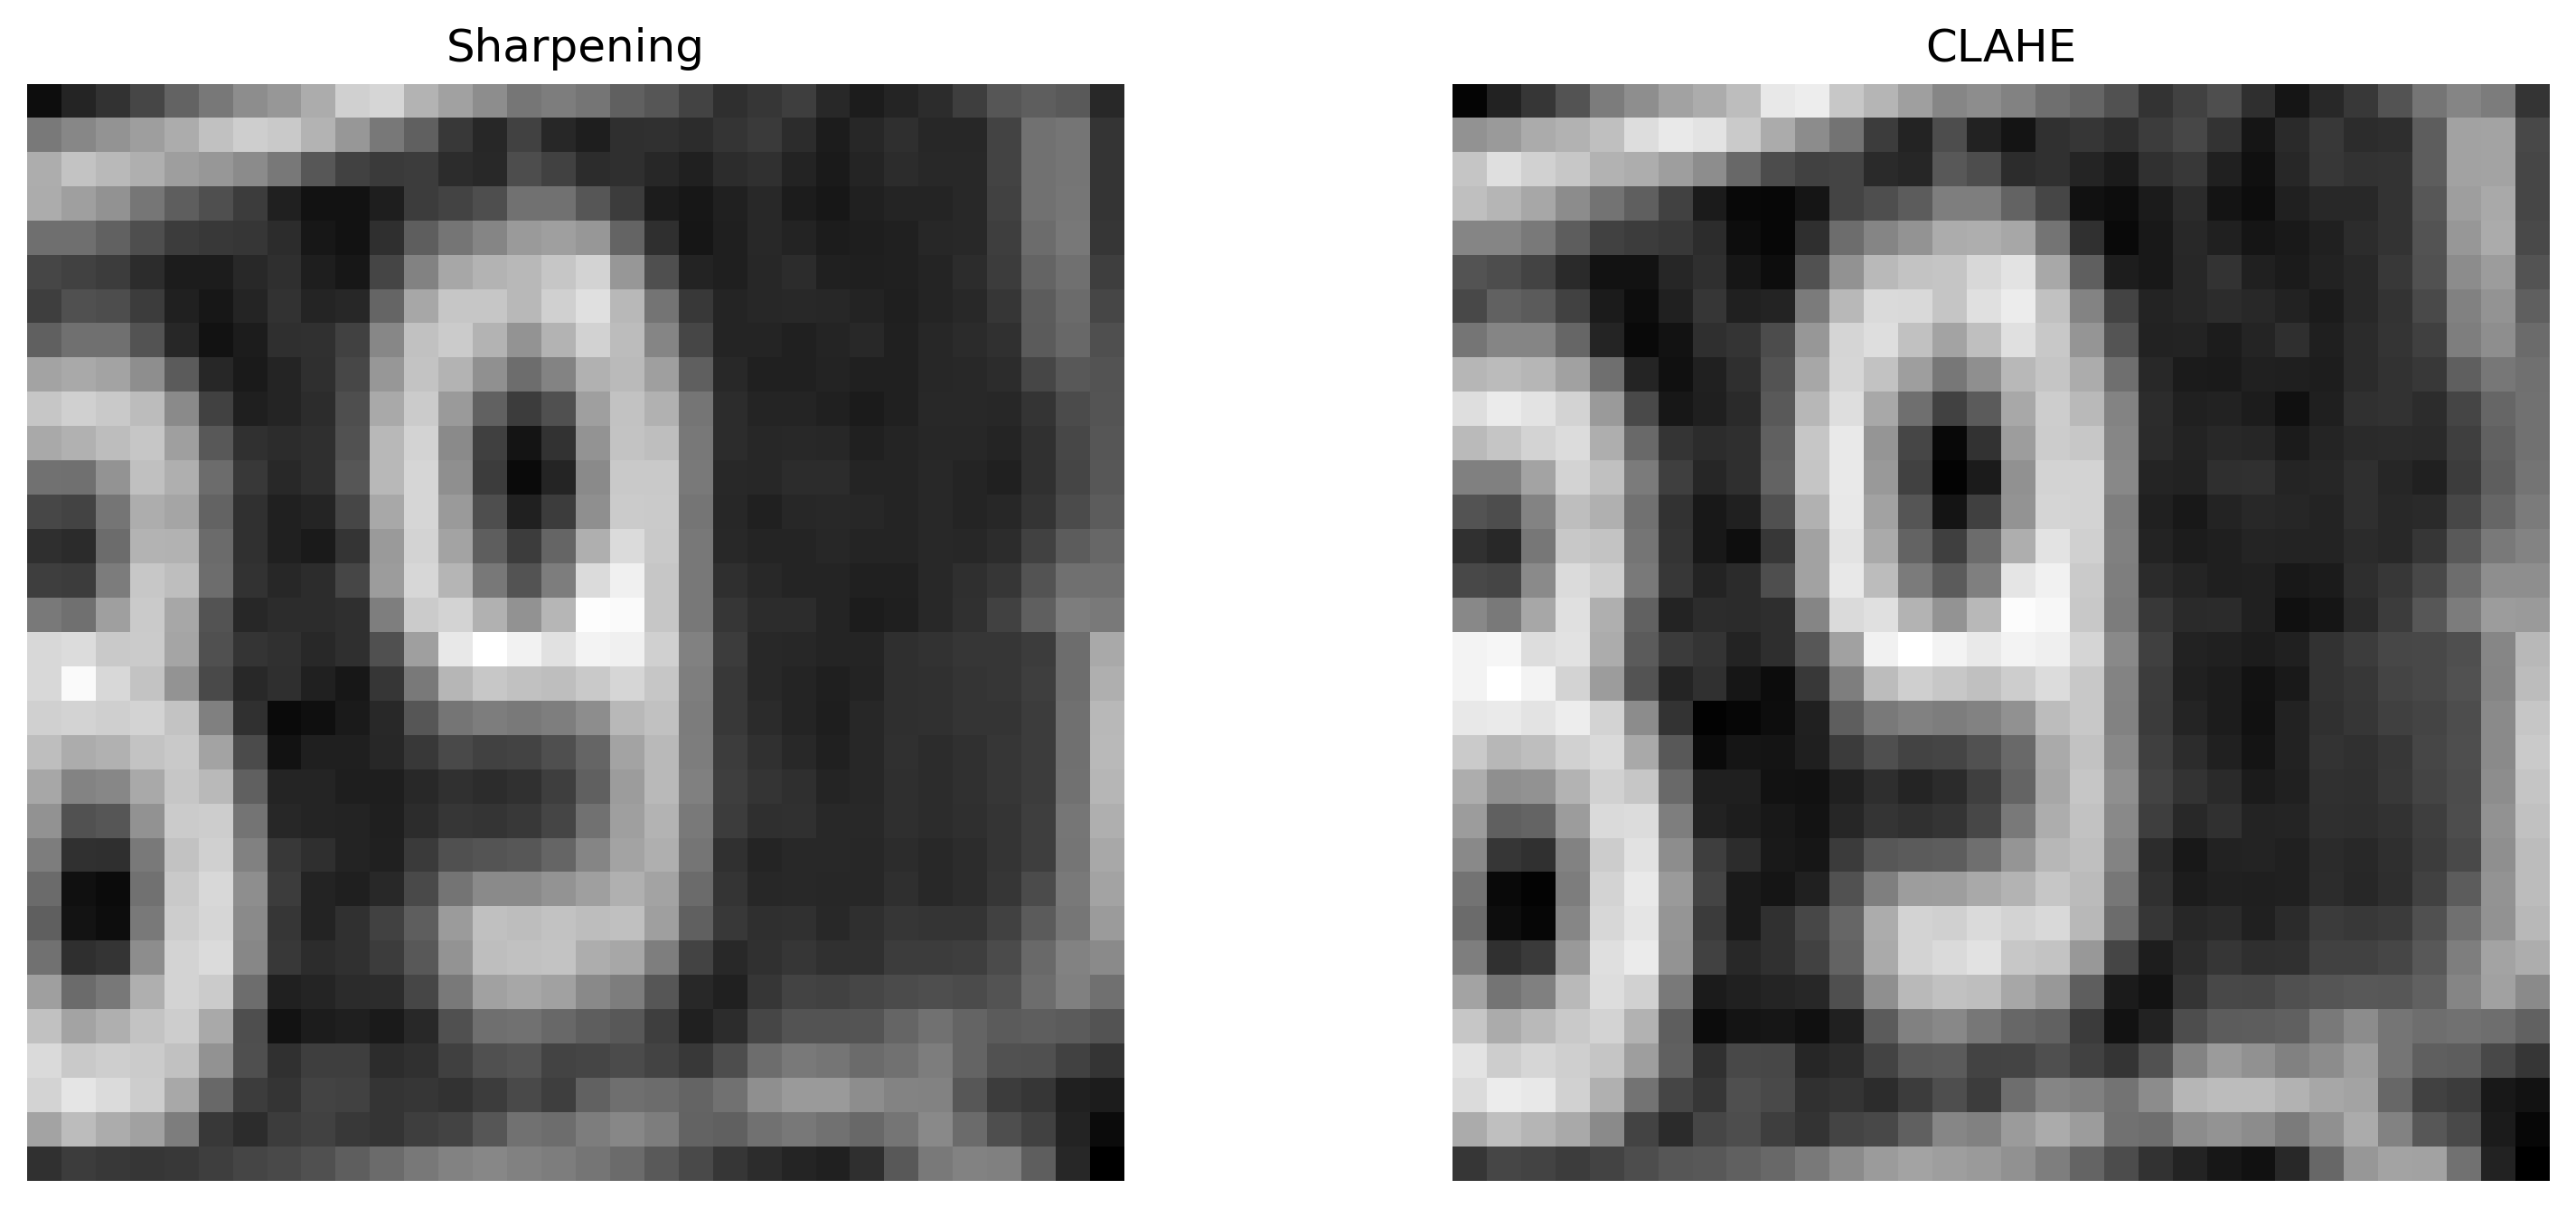
\includegraphics[width=\linewidth]{figures/row_2_images.png}
        \caption{Sharpening y CLAHE}
        \label{fig:row_2}
\end{figure}

\begin{figure}[H]
        \centering
        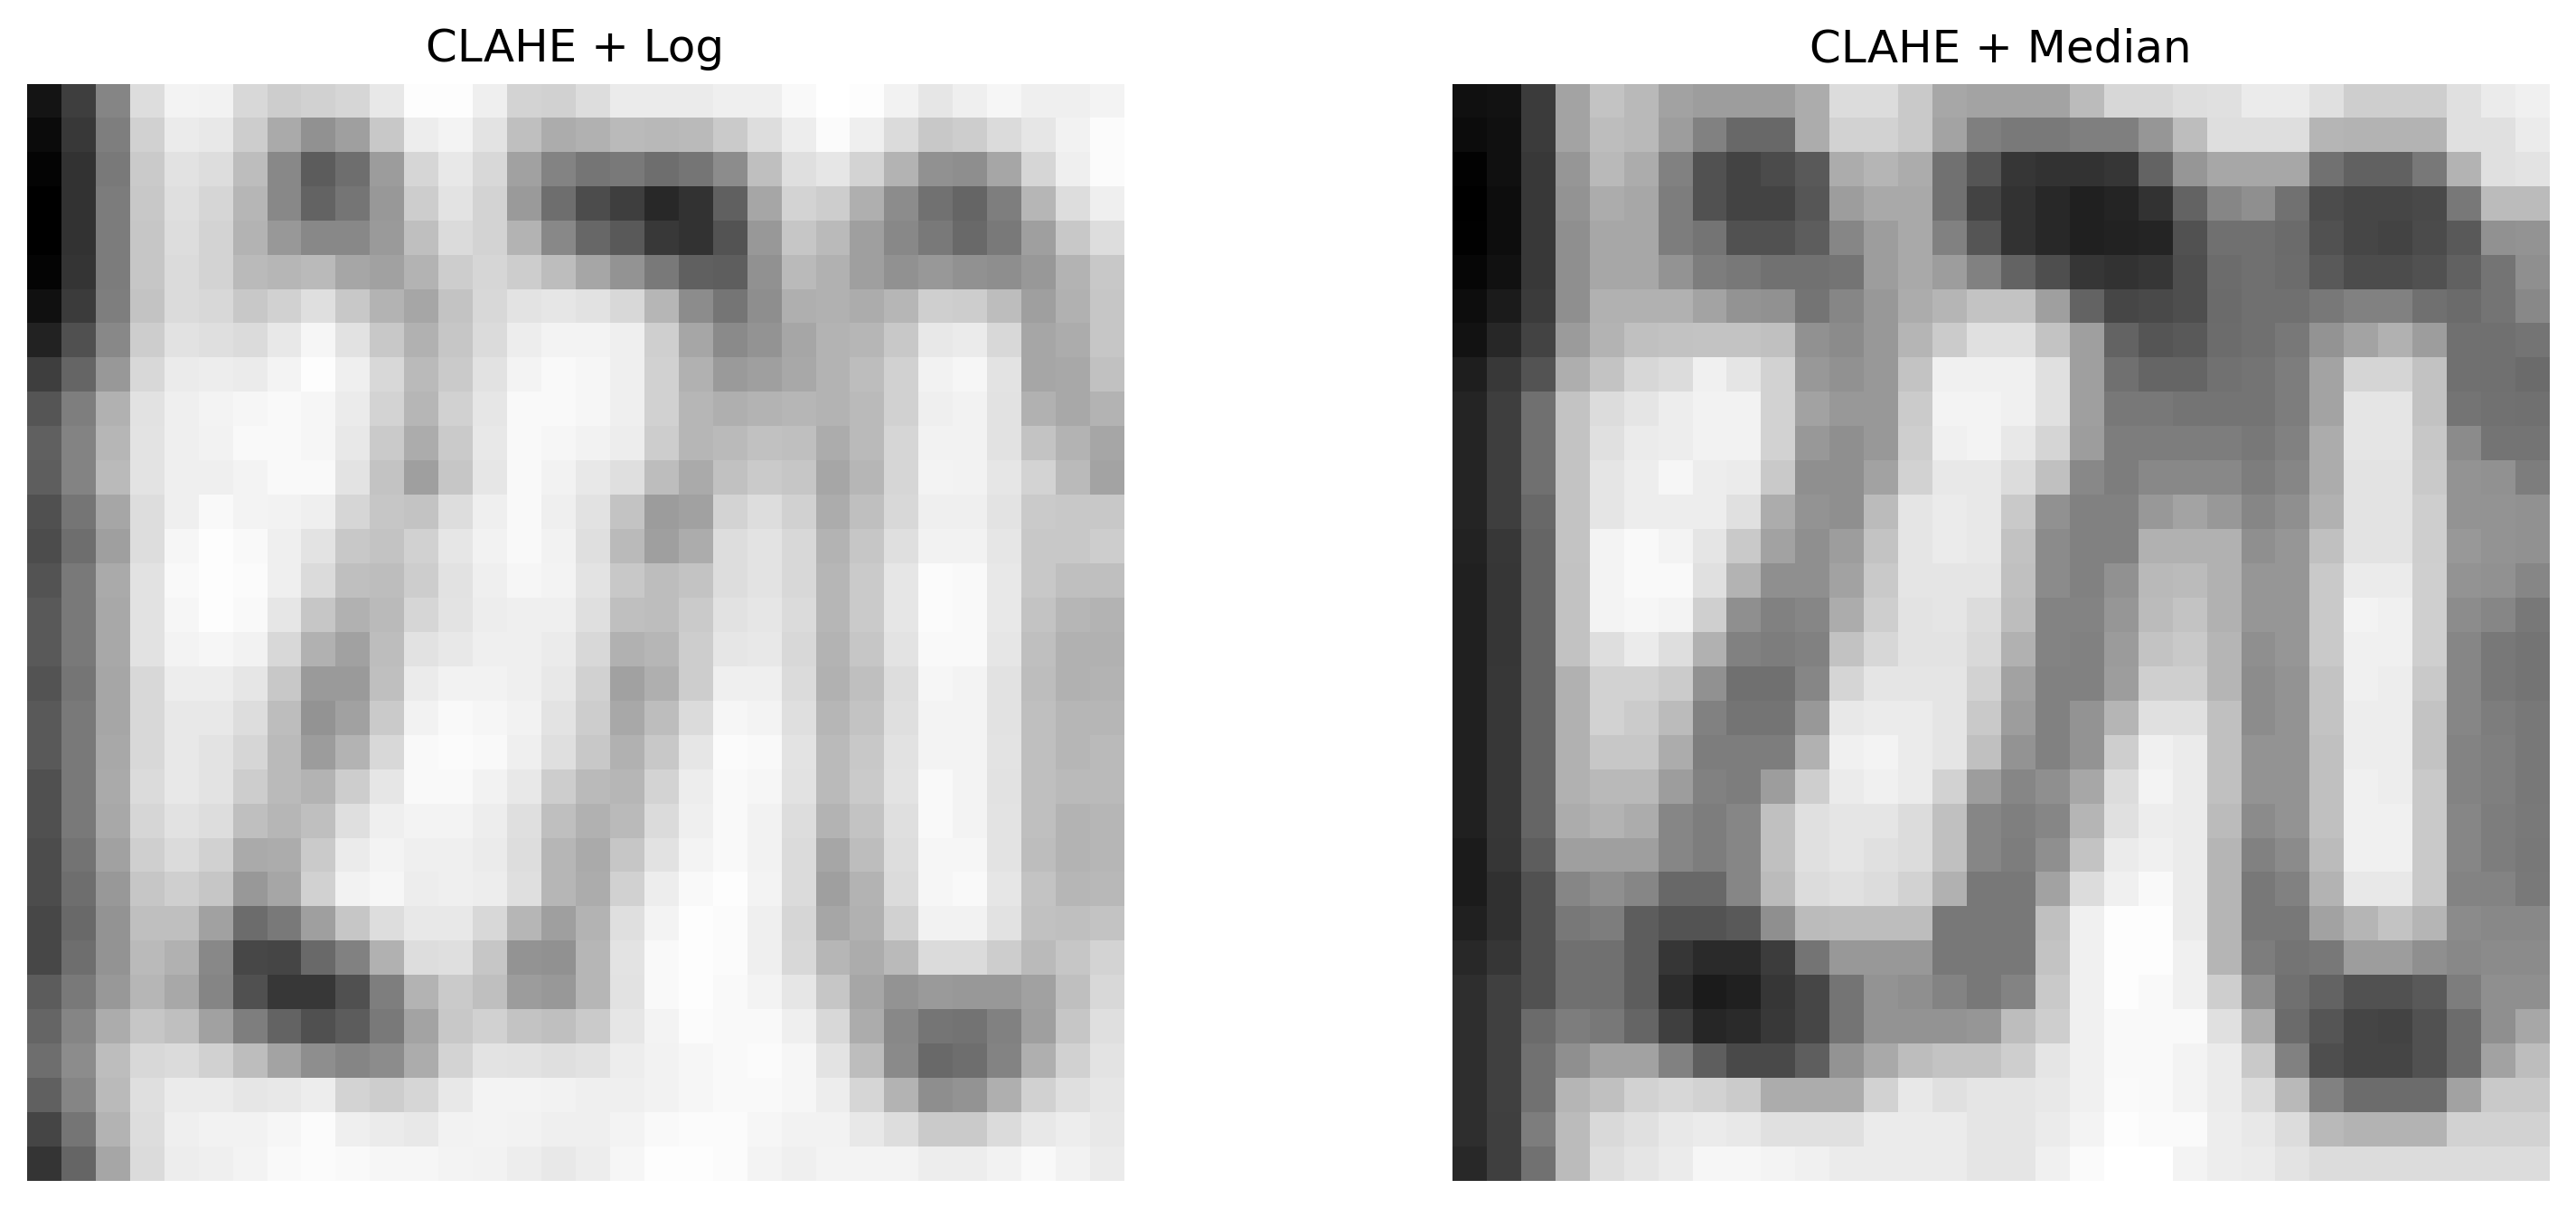
\includegraphics[width=\linewidth]{figures/row_3_images.png}
        \caption{Transformaciones Logarítmicas y Mediana a imagen CLAHE}
        \label{fig:row_3}
\end{figure}

\begin{figure}[H]
        \centering
        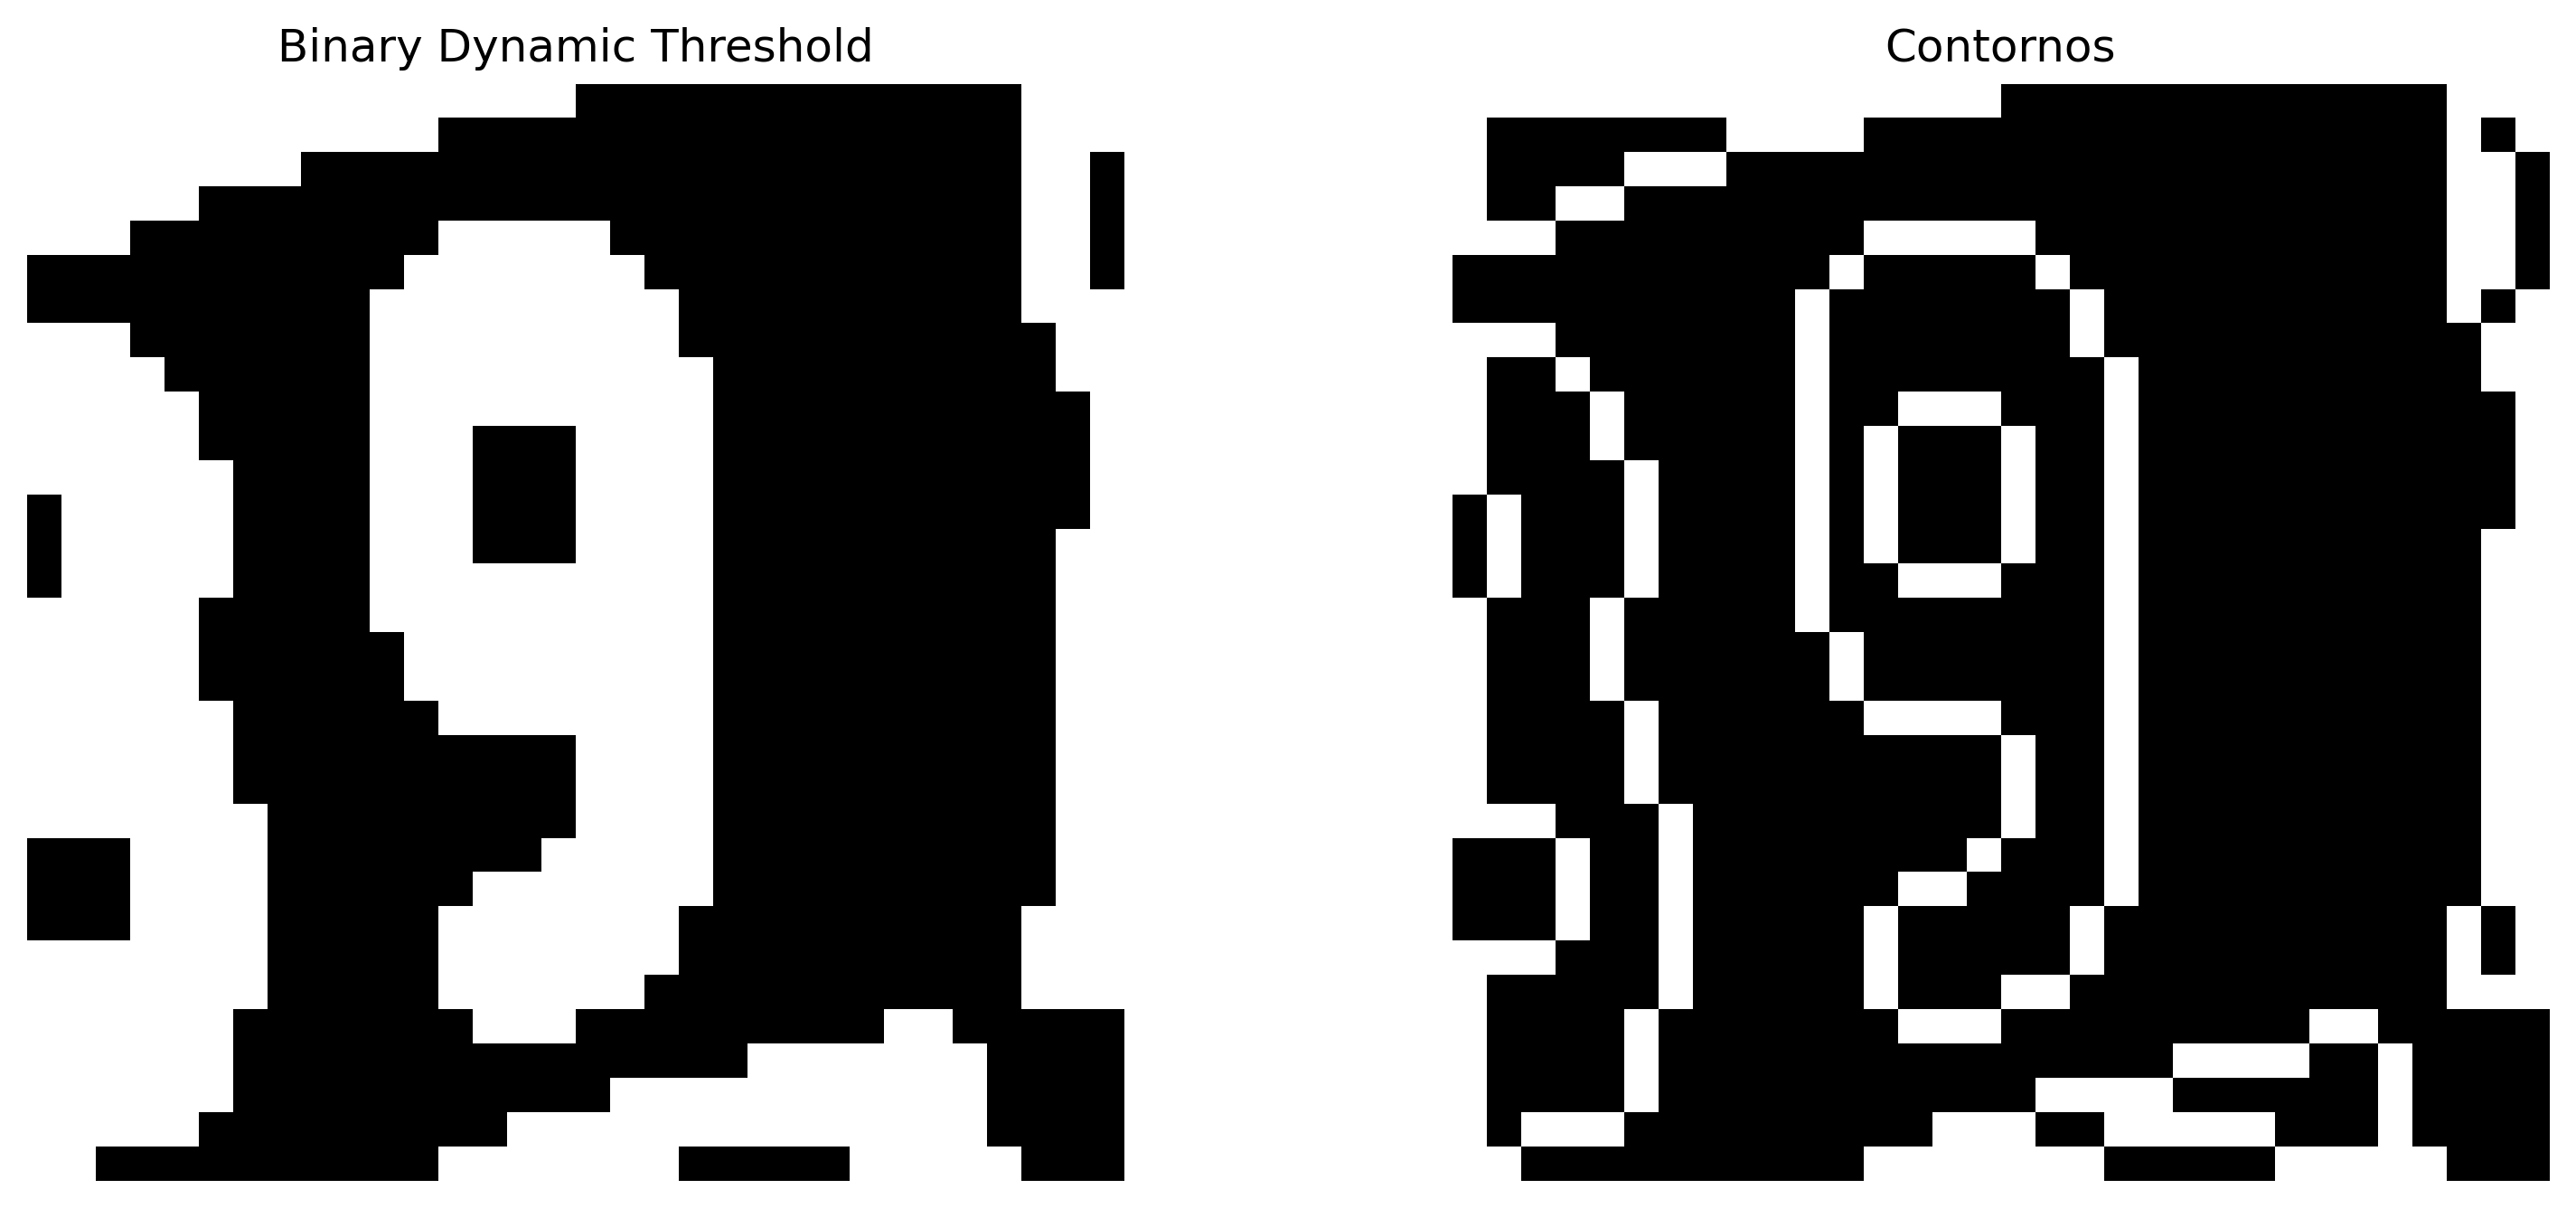
\includegraphics[width=\linewidth]{figures/row_4_images.png}
        \caption{Binary Dynamic Threshold y extracción de contornos}
        \label{fig:row_4}
\end{figure}

\begin{figure}[H]
        \centering
        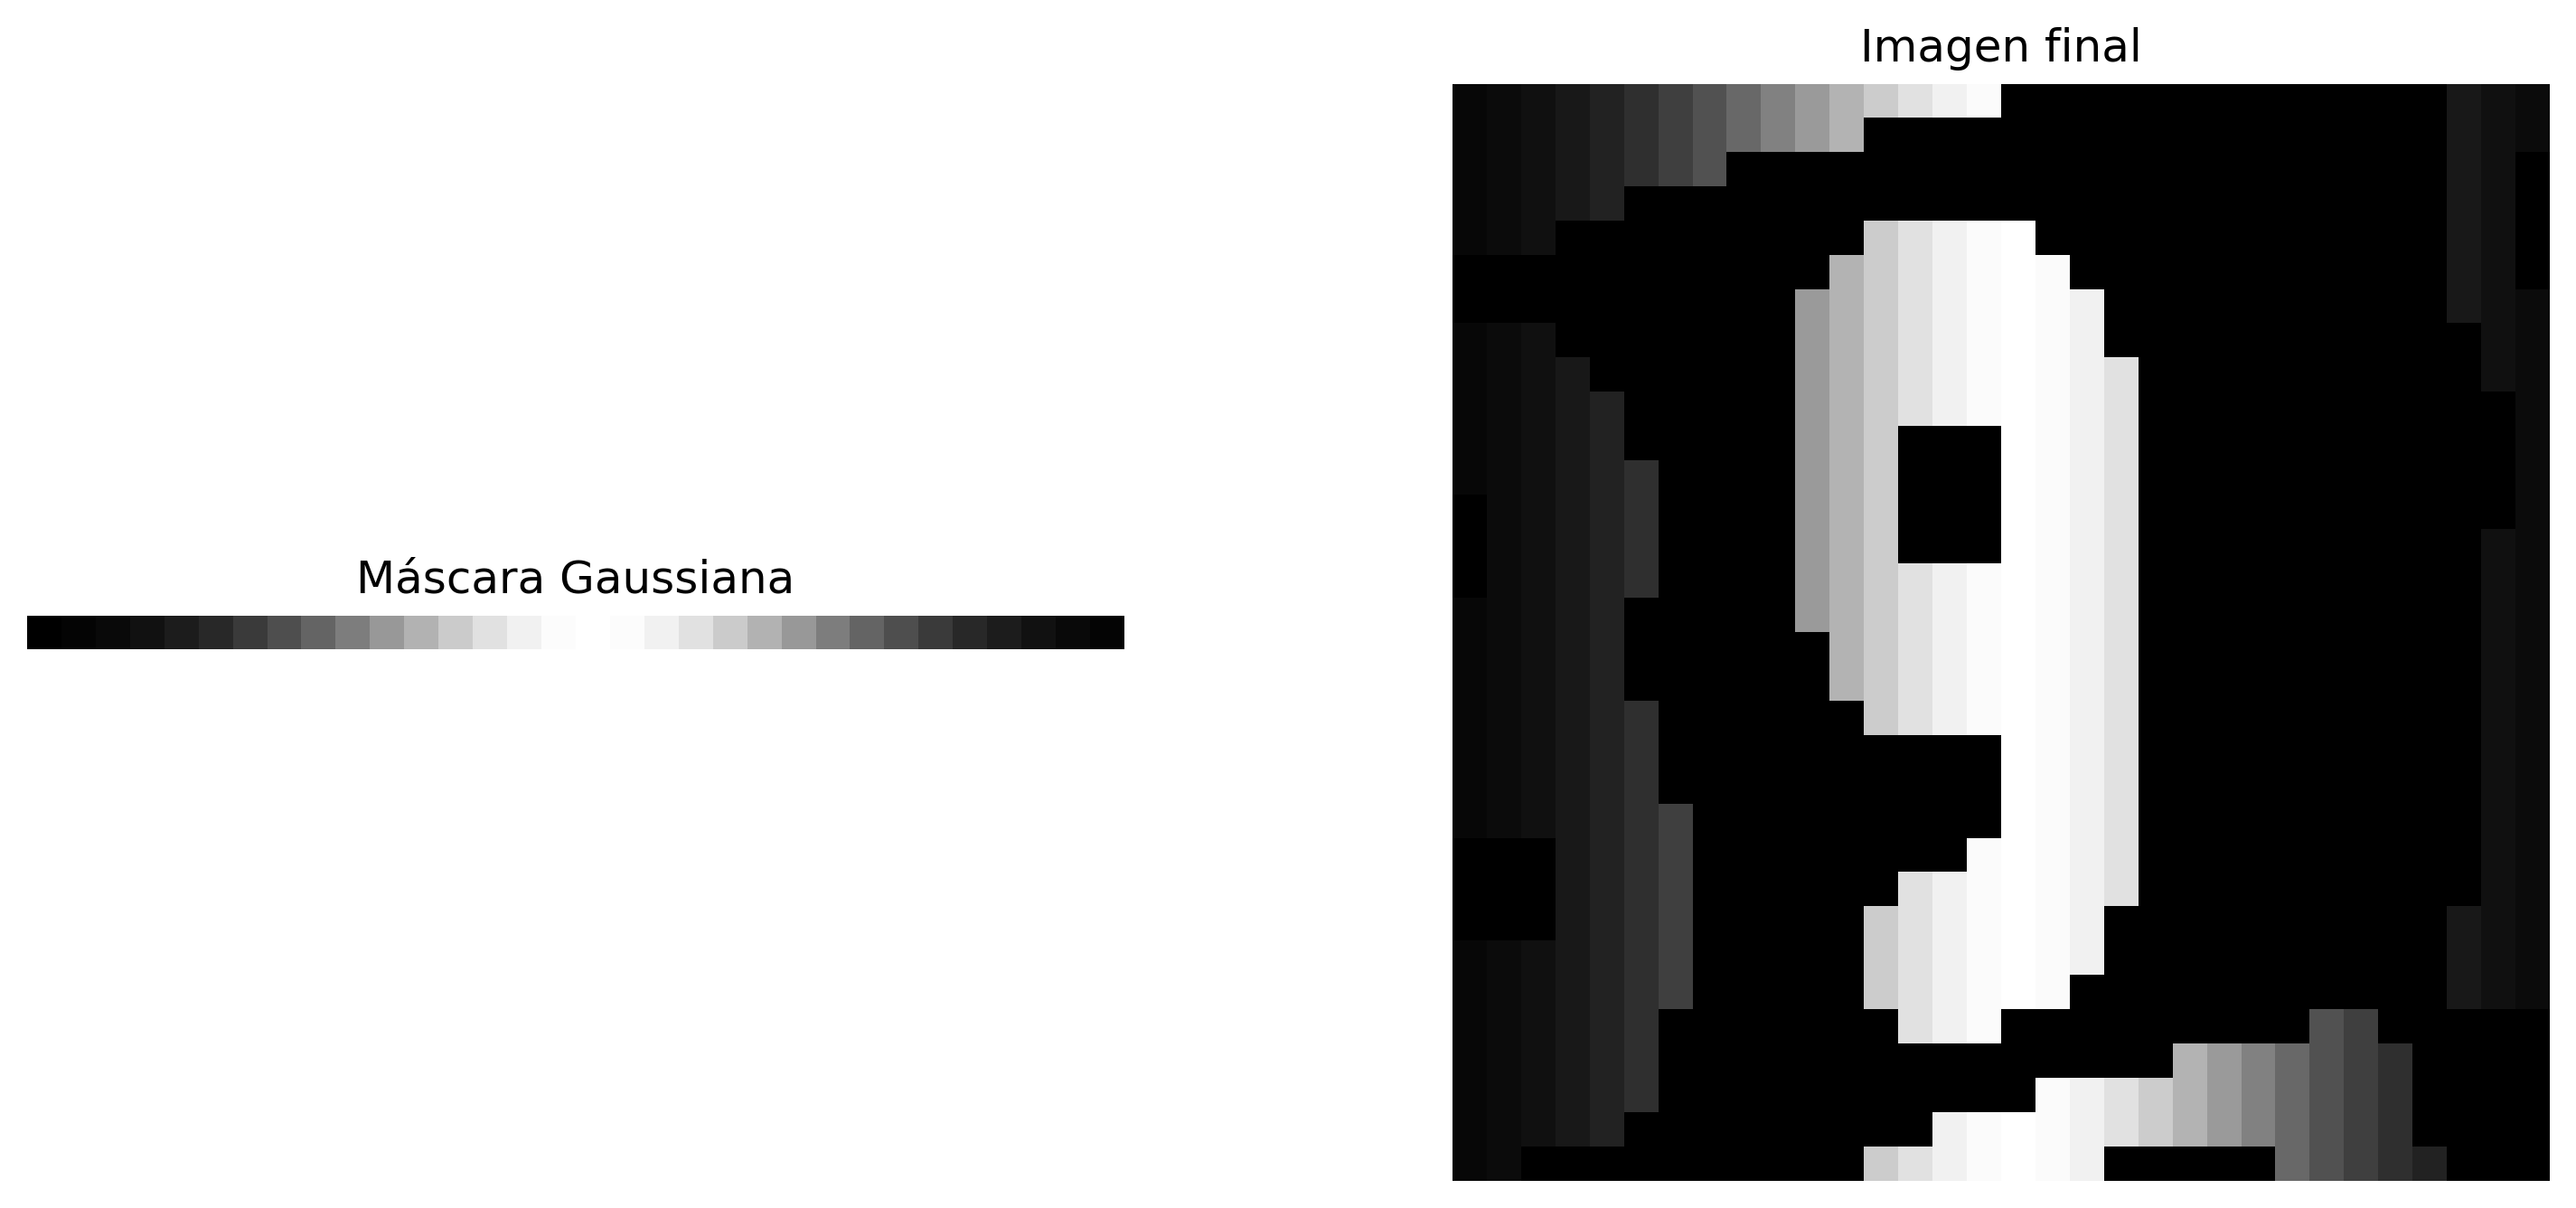
\includegraphics[width=\linewidth]{figures/row_5_images.png}
        \caption{Filtro Gaussiano e imagen pre-procesada final}
        \label{fig:row_5}
\end{figure}

\subsubsection{Reducción de dimensiones}

Debido a la excesiva cantidad de dimensiones (1024) aún con las transformaciones antes mencionadas, se propone utilizar los siguientes métodos para reducir este número:
\begin{itemize}
        \item PCA\cite{scikit-learn_pca}
        \item UMAP\cite{umap-learn}
        \item tSNE\cite{scikit-learn-tsne}
\end{itemize}

En los 3 casos se hicieron reducciones a 2 y 3 dimensiones, sin embargo, no fue posible encontrar separaciones bien definidas, lo que sugiere que se necesitan más dimensiones para observar estos datos. UMAP aparenta tener la mejor separación.

\begin{figure}[H]
        \centering
        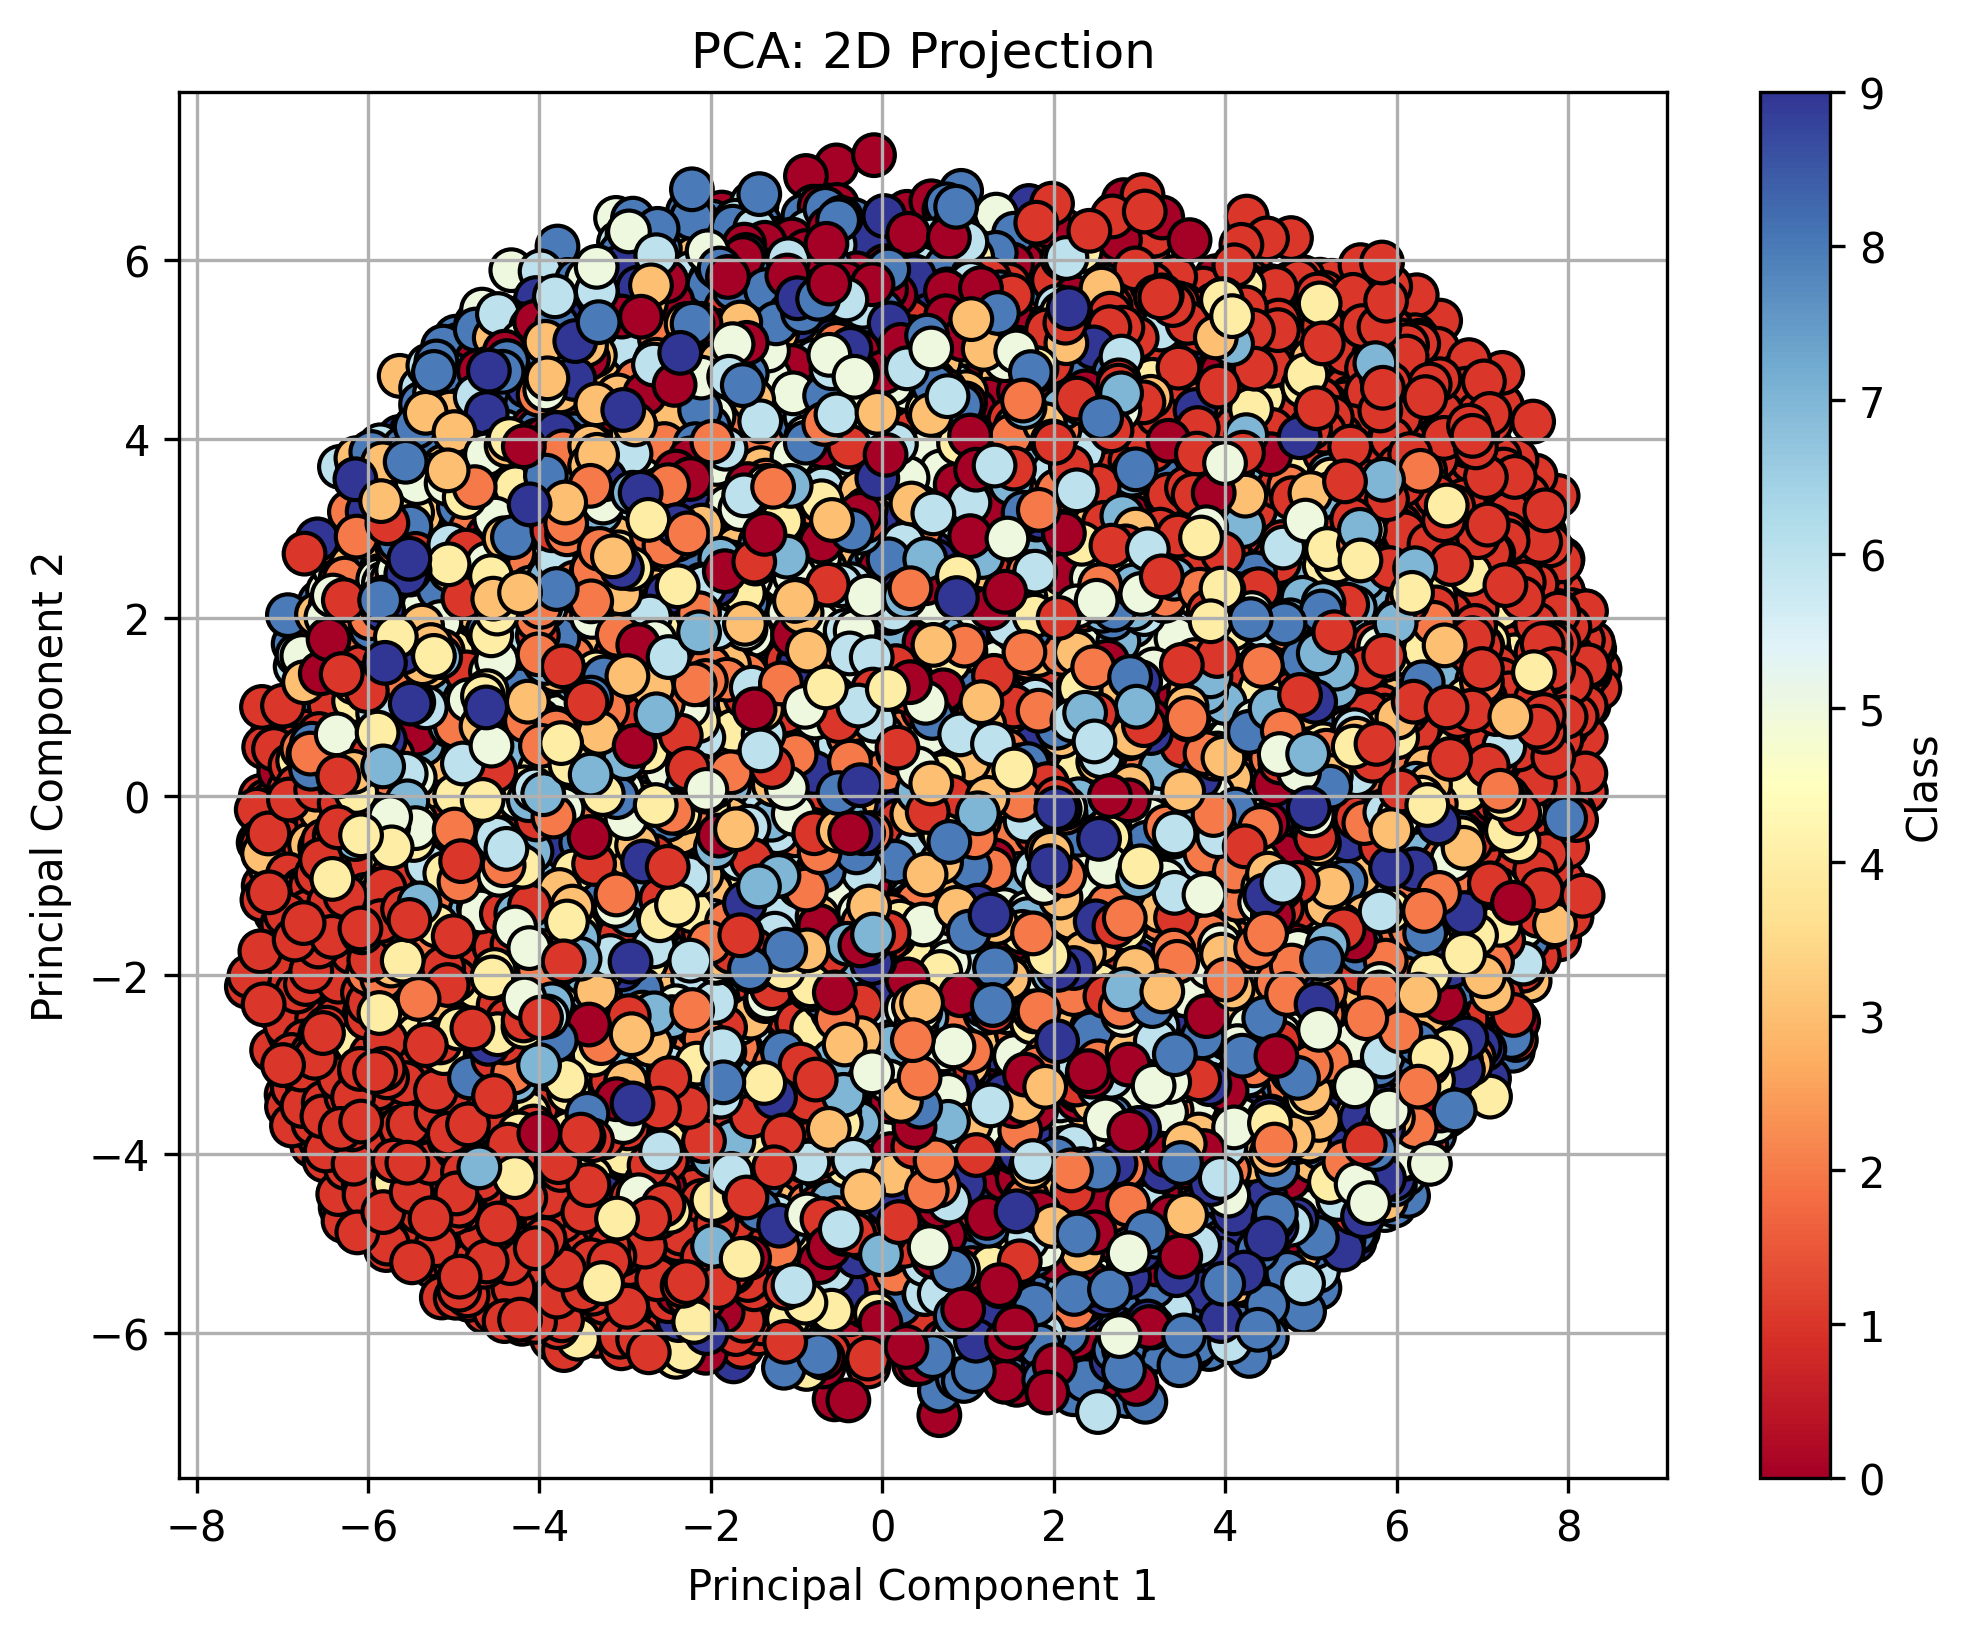
\includegraphics[width=0.9\linewidth]{figures/pca_2d_projection.png}
        \caption{PCA: 2D}
        \label{fig:pca_2d}
\end{figure}

\begin{figure}[H]
        \centering
        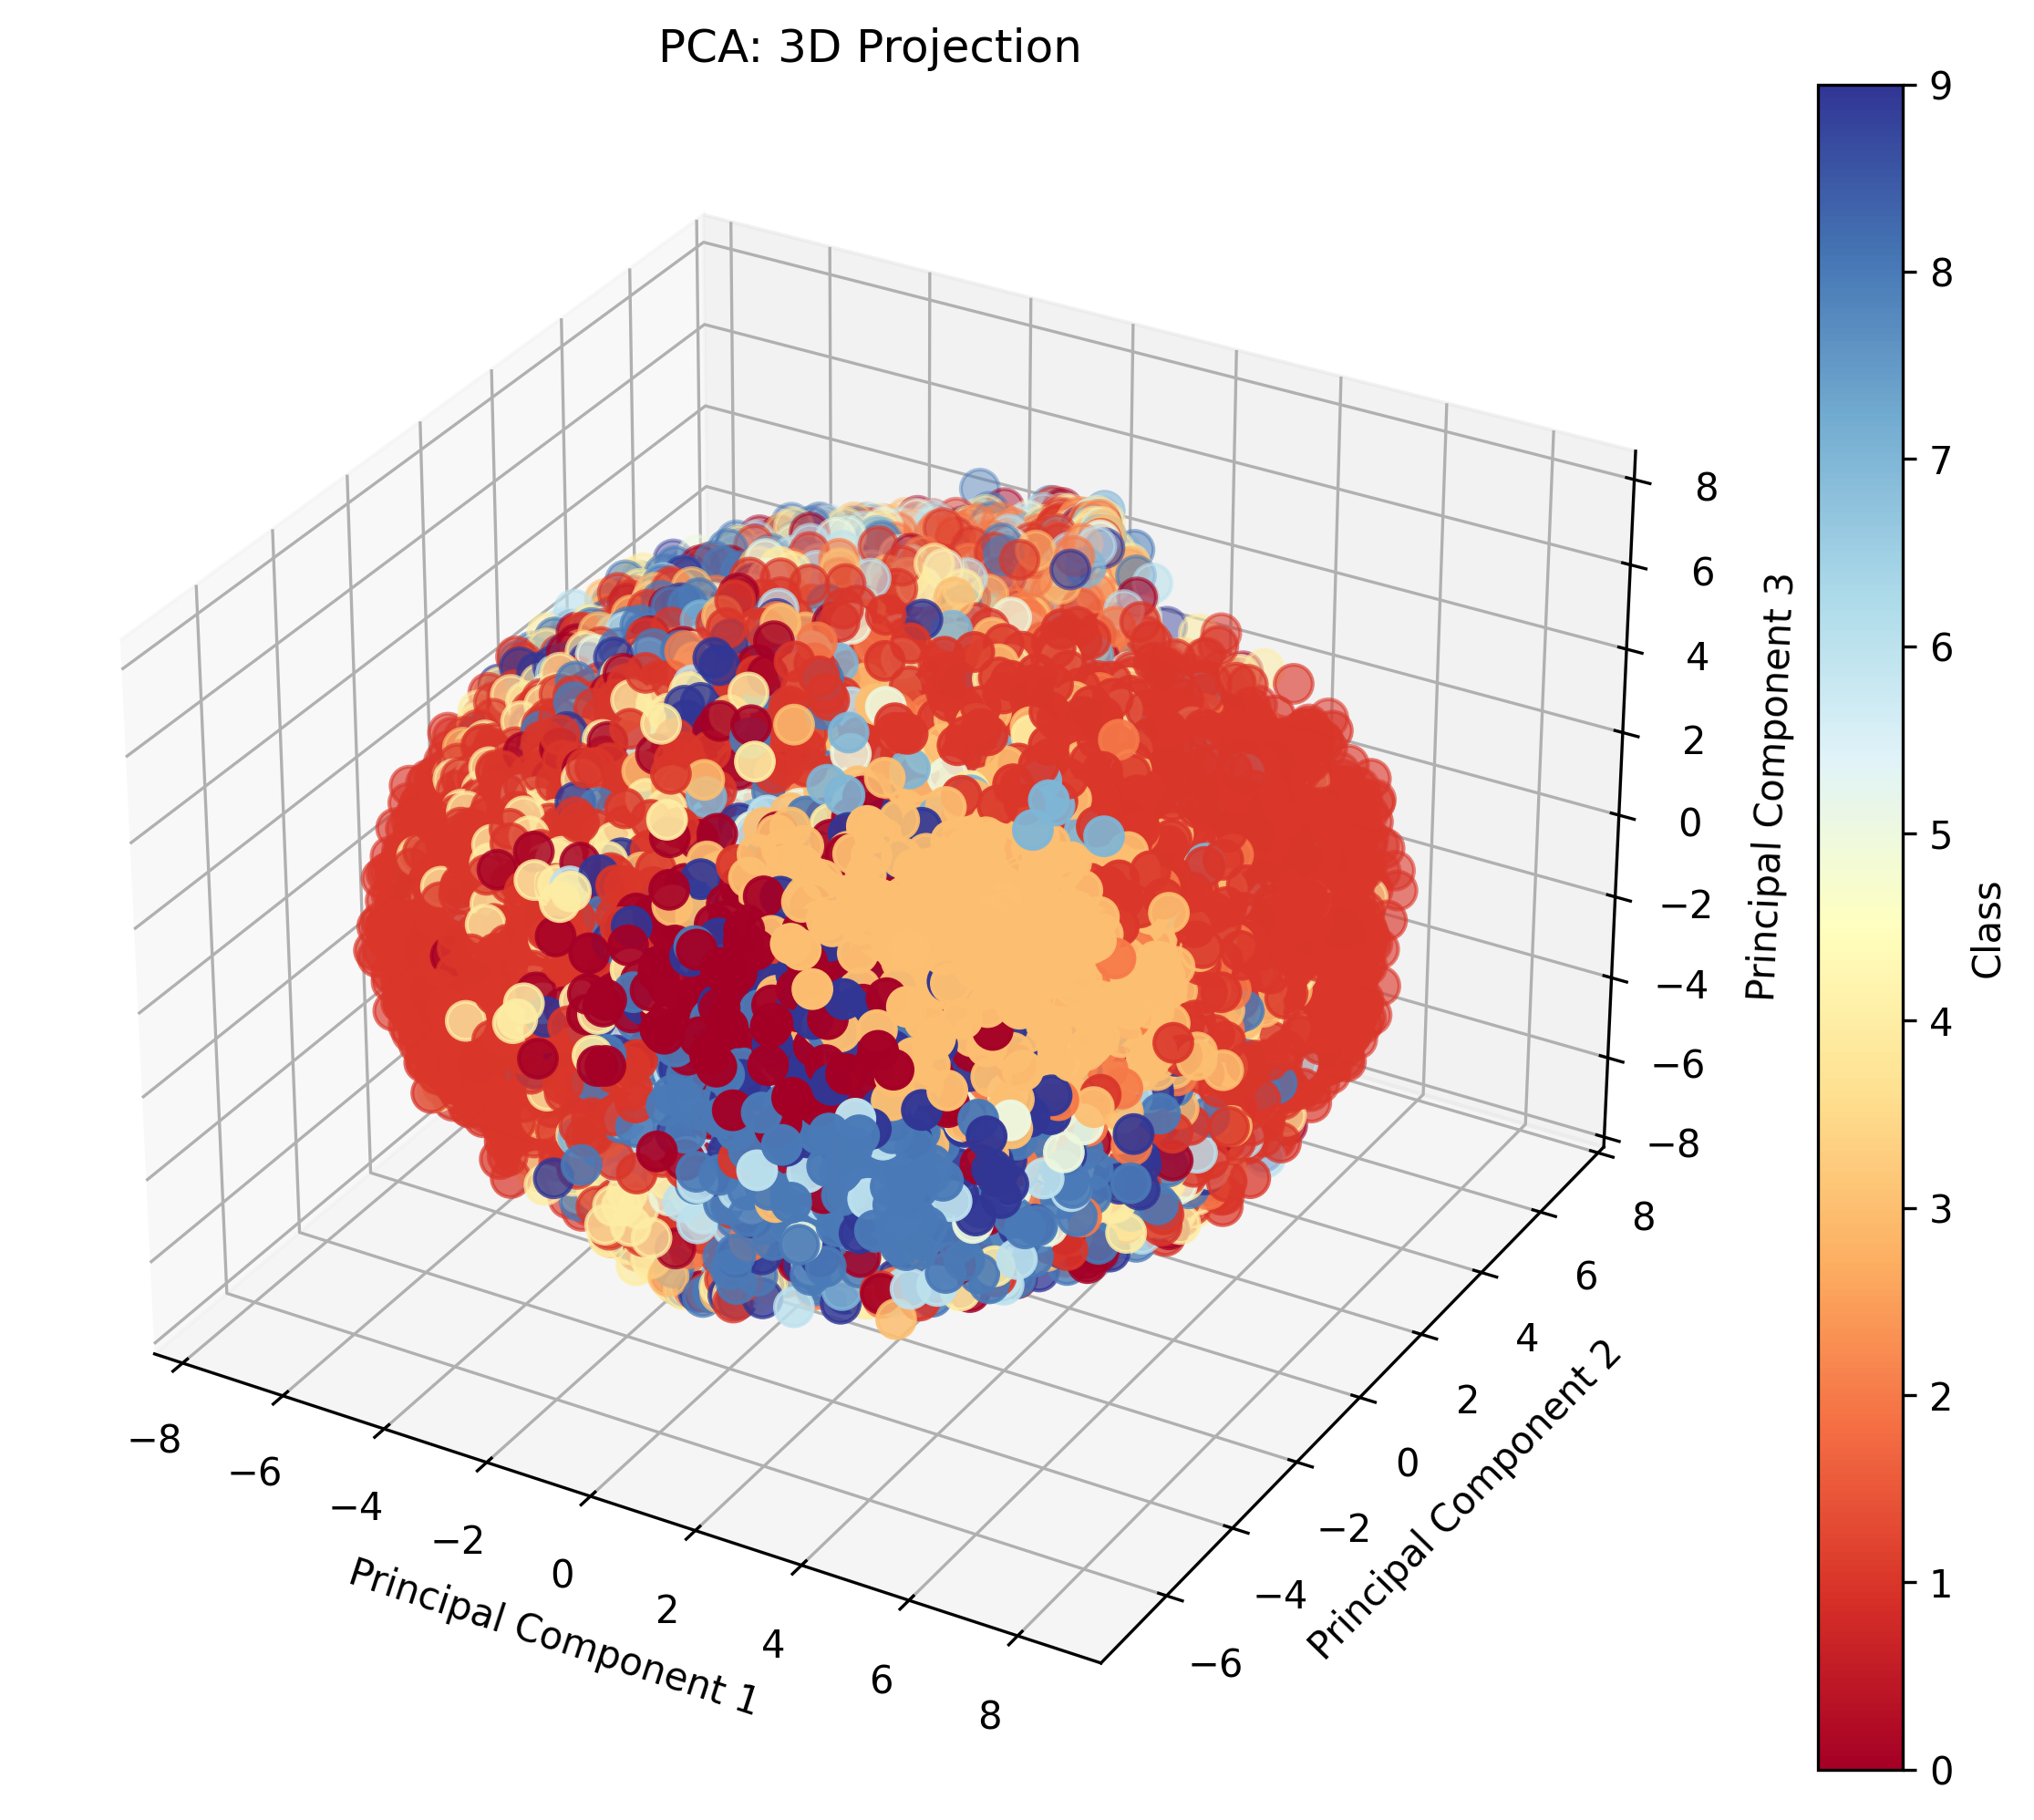
\includegraphics[width=0.9\linewidth]{figures/pca_3d_projection.png}
        \caption{PCA: 3D}
        \label{fig:pca_3d}
\end{figure}

\begin{figure}[hbt!]
        \centering
        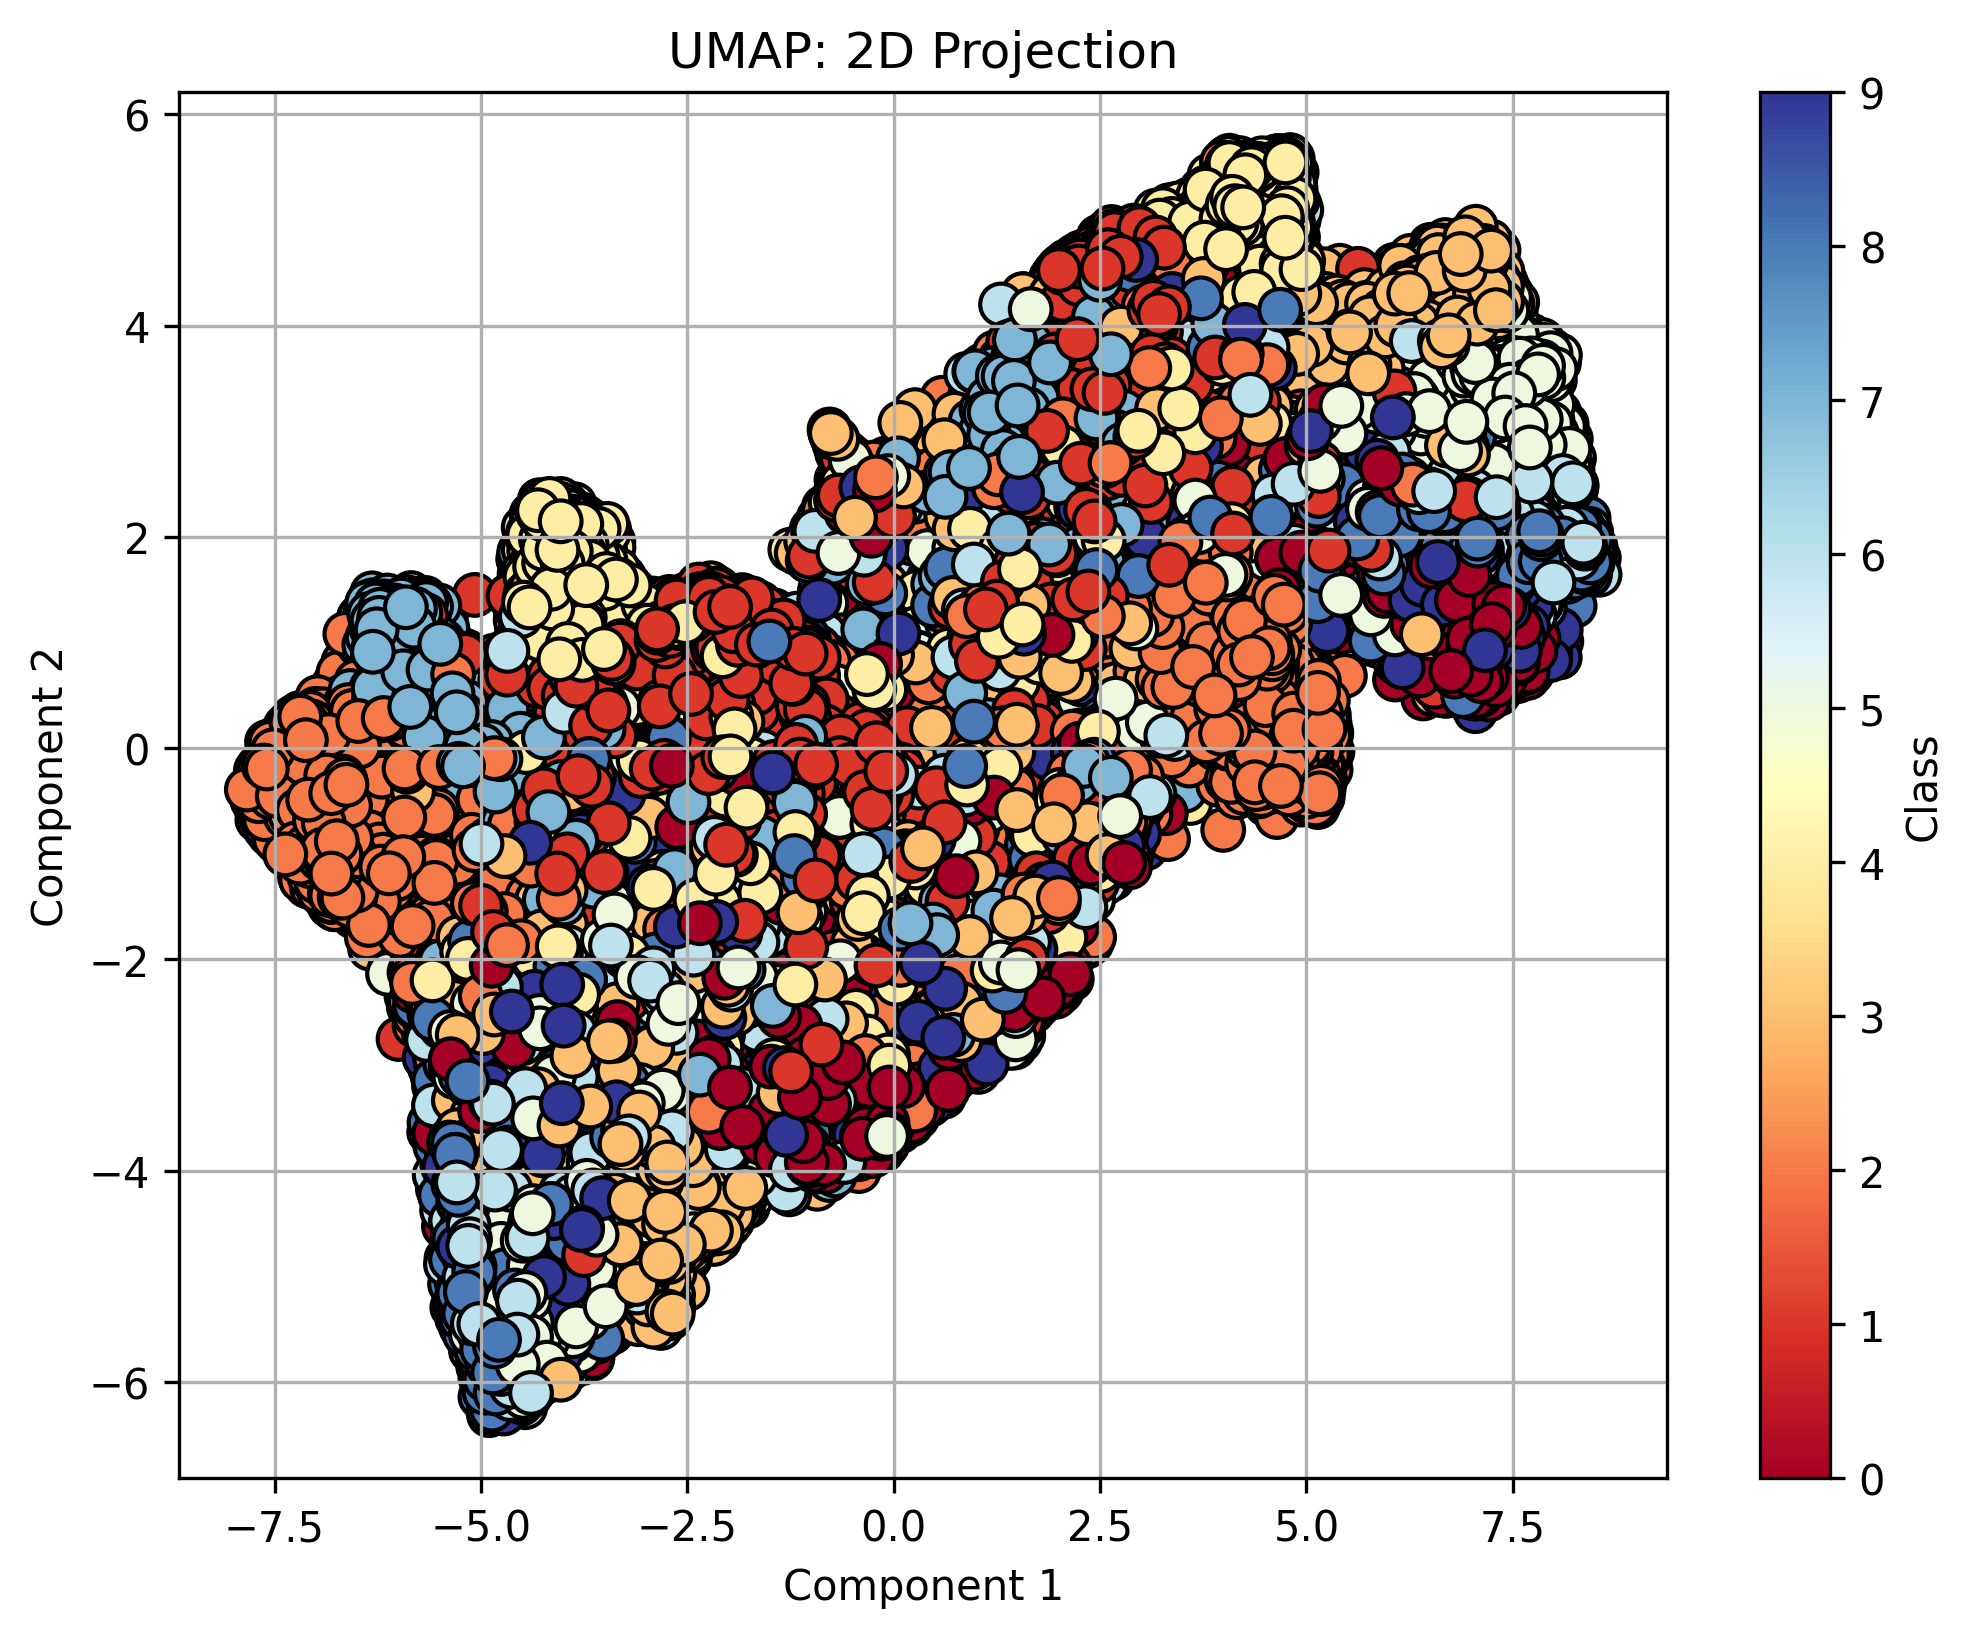
\includegraphics[width=0.9\linewidth]{figures/umap_2d_projection.png}
        \caption{UMAP: 2D}
        \label{fig:umap_2d}
\end{figure}
\vspace{-10pt}
\begin{figure}[H]
        \centering
        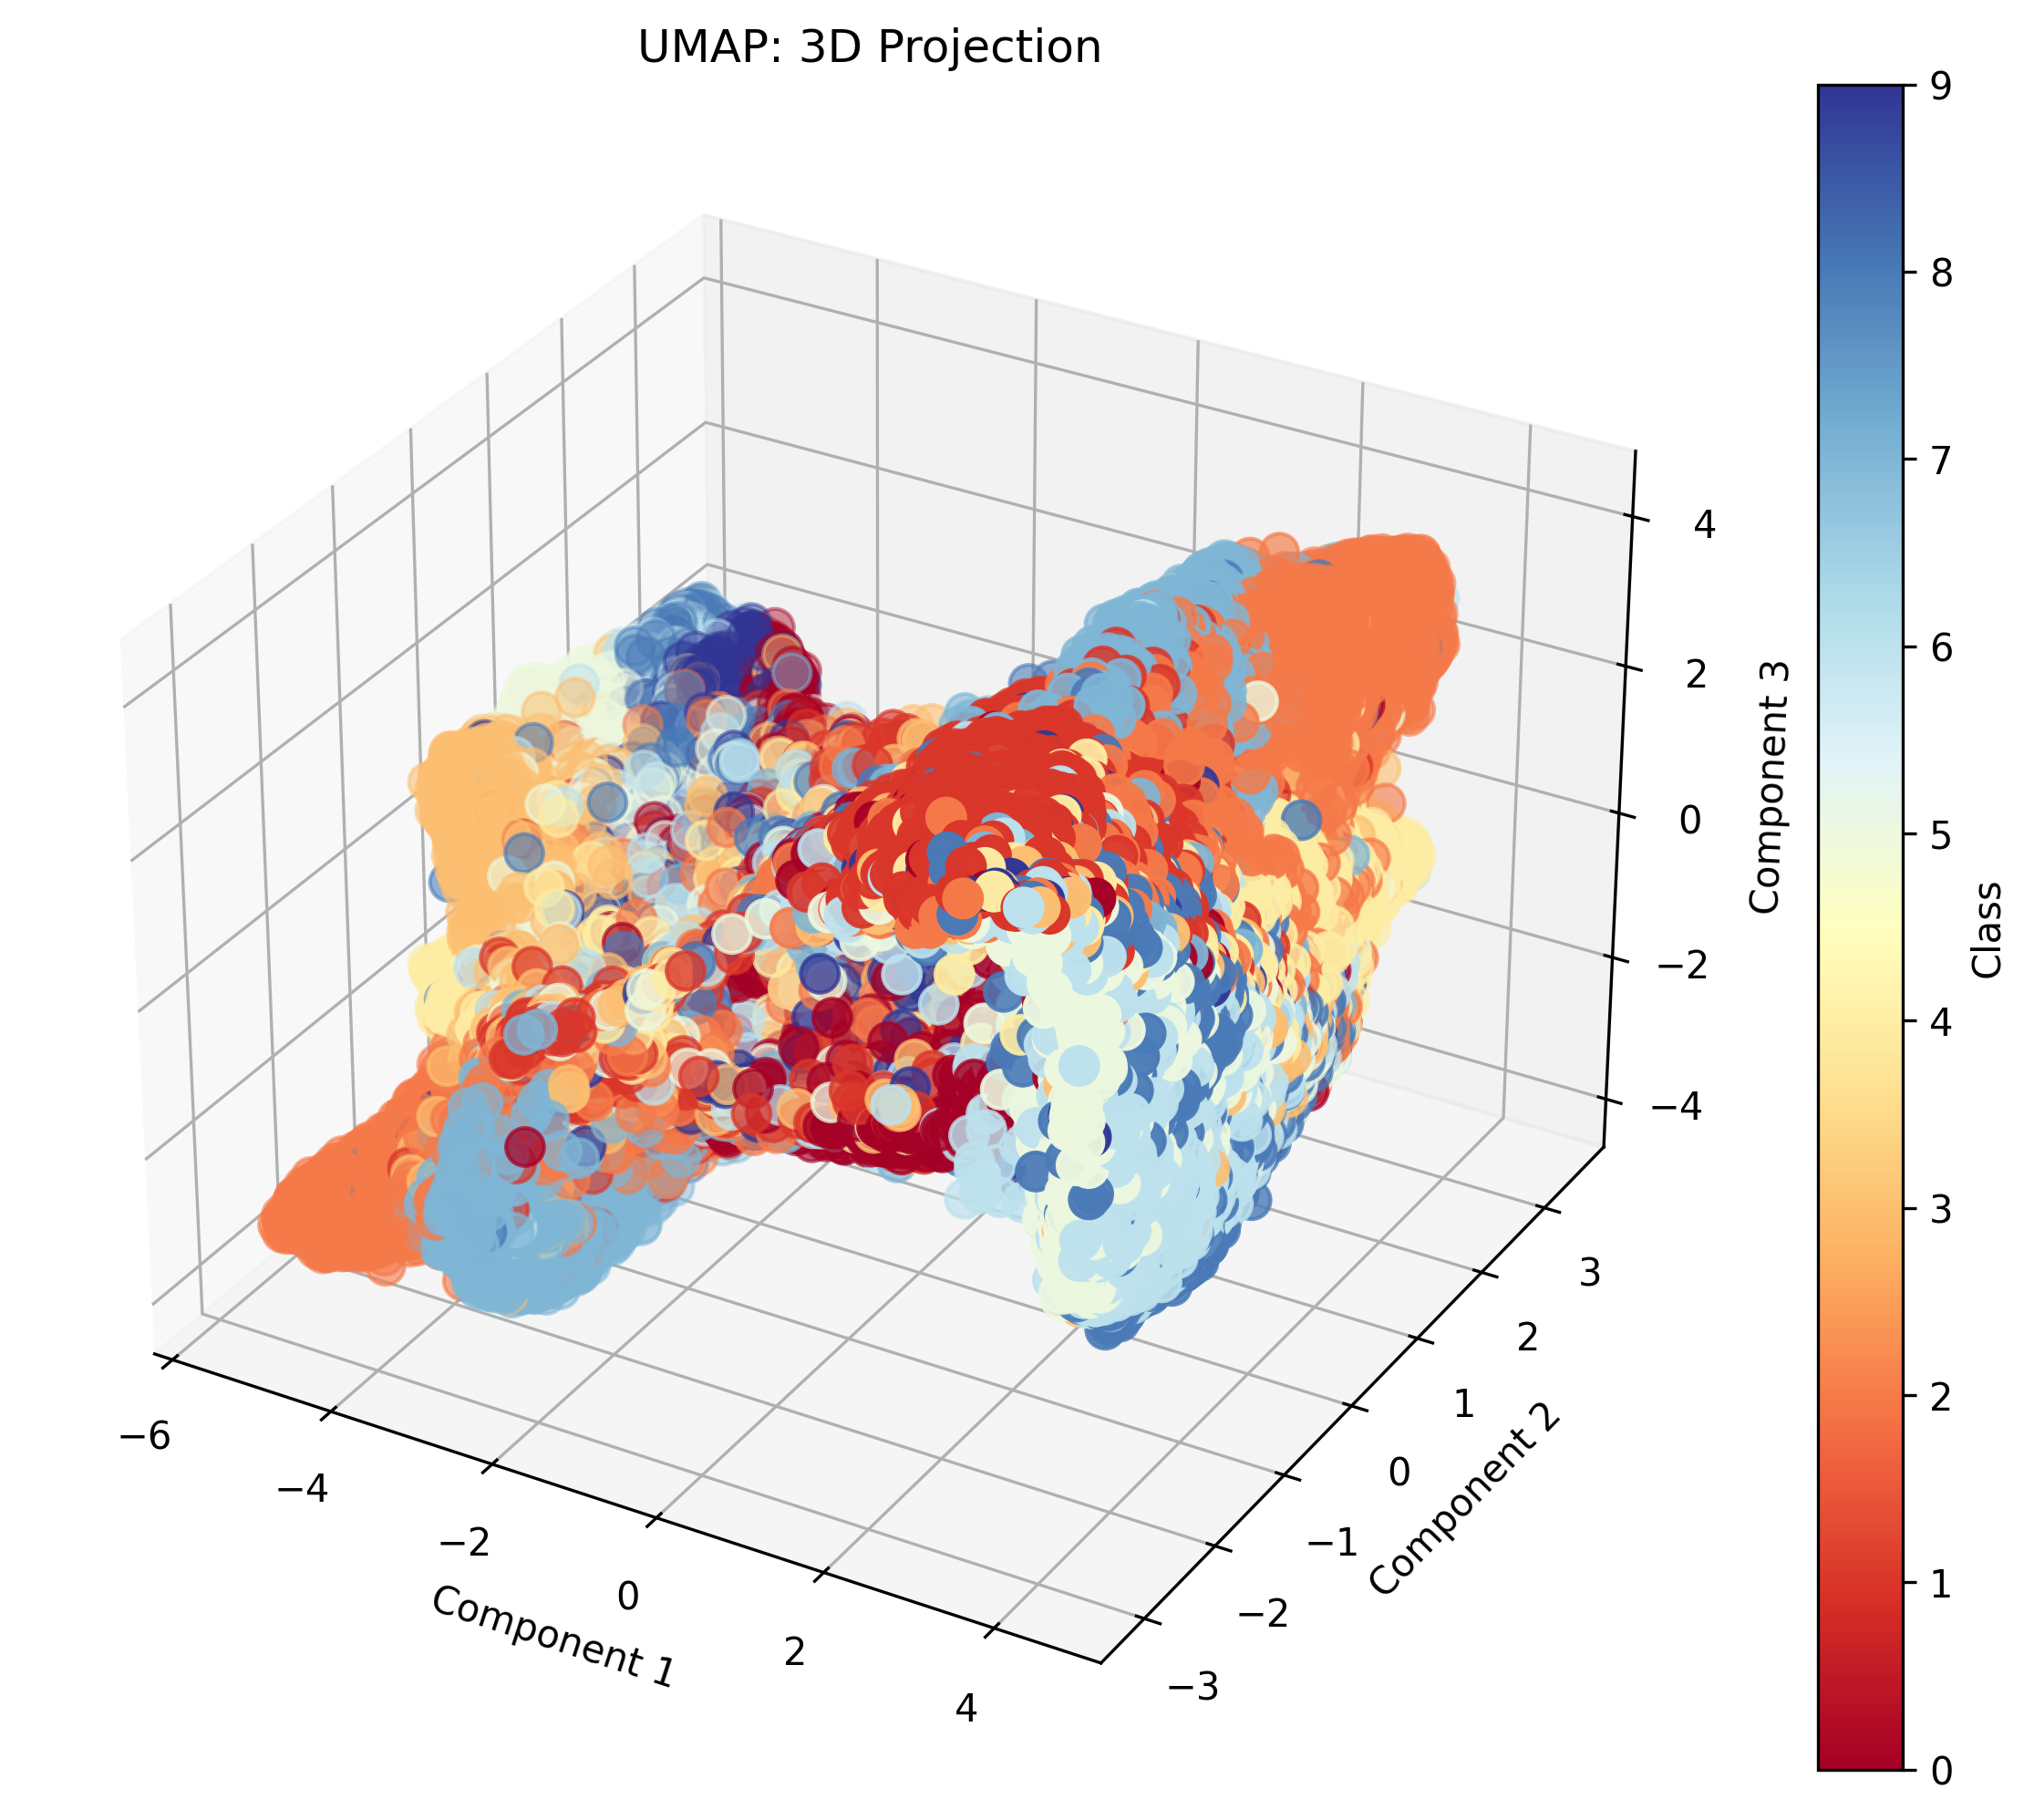
\includegraphics[width=0.9\linewidth]{figures/umap_3d_projection.png}
        \caption{UMAP: 3D}
        \label{fig:umap_3d}
\end{figure}

\begin{figure}[H]
        \centering
        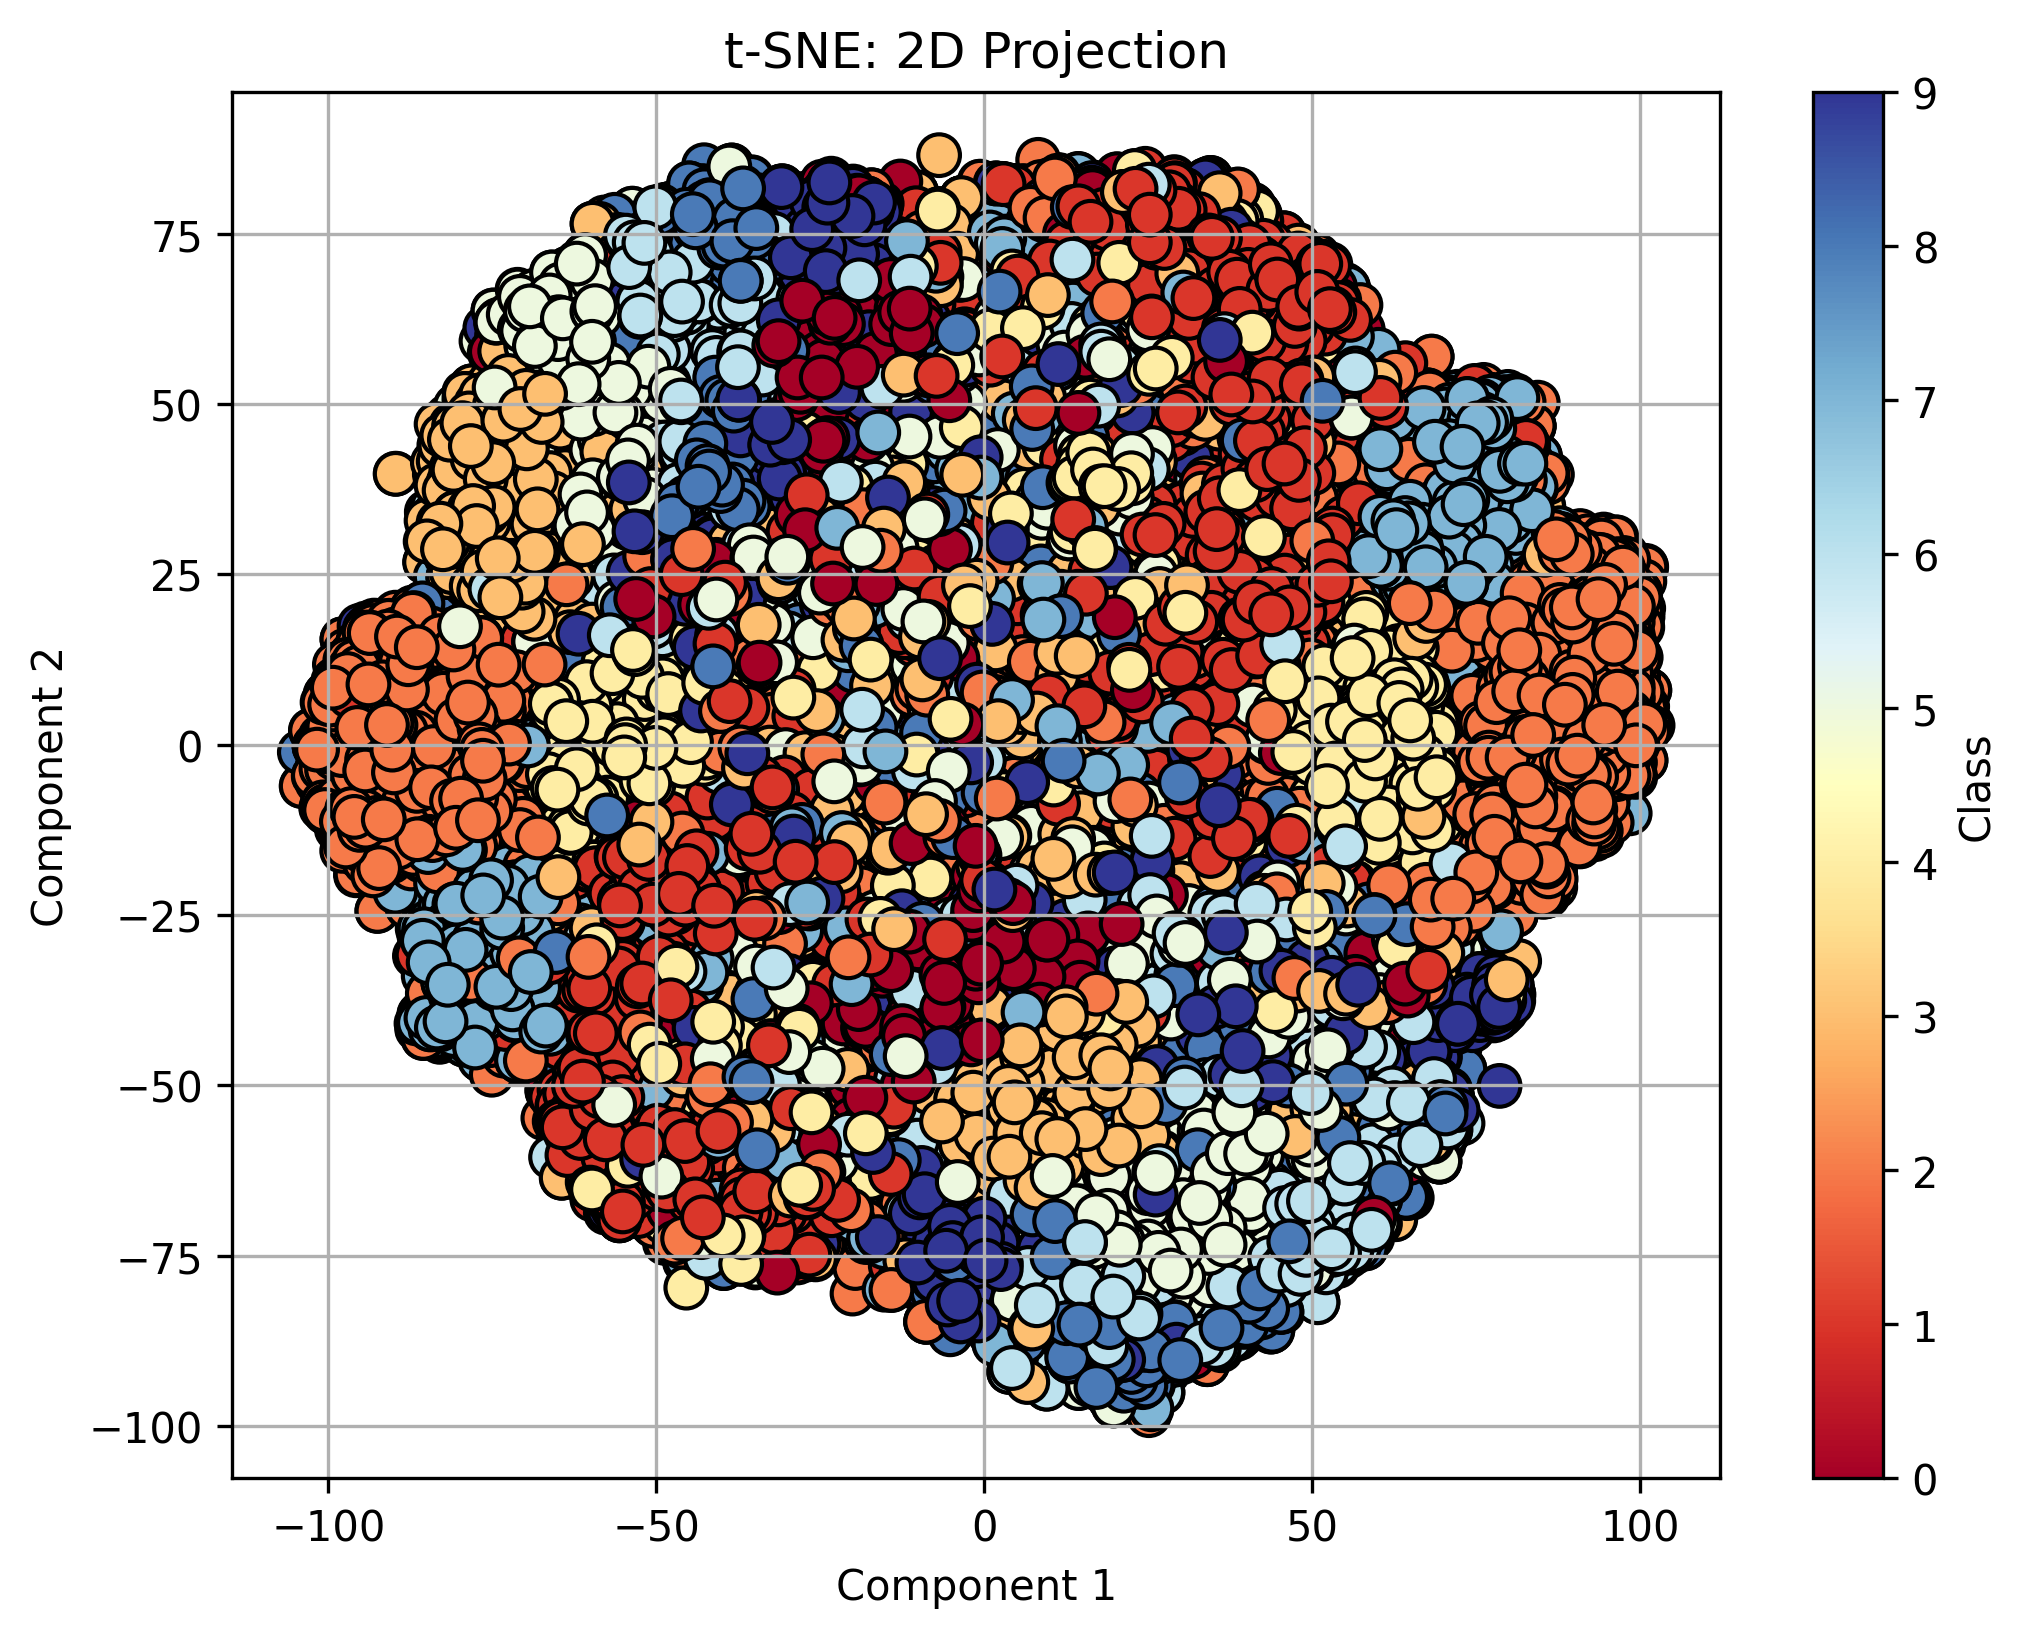
\includegraphics[width=0.9\linewidth]{figures/tsne_2d_projection.png}
        \caption{tSNE: 2D}
        \label{fig:tsne_2d}
\end{figure}
\begin{figure}[H]
        \centering
        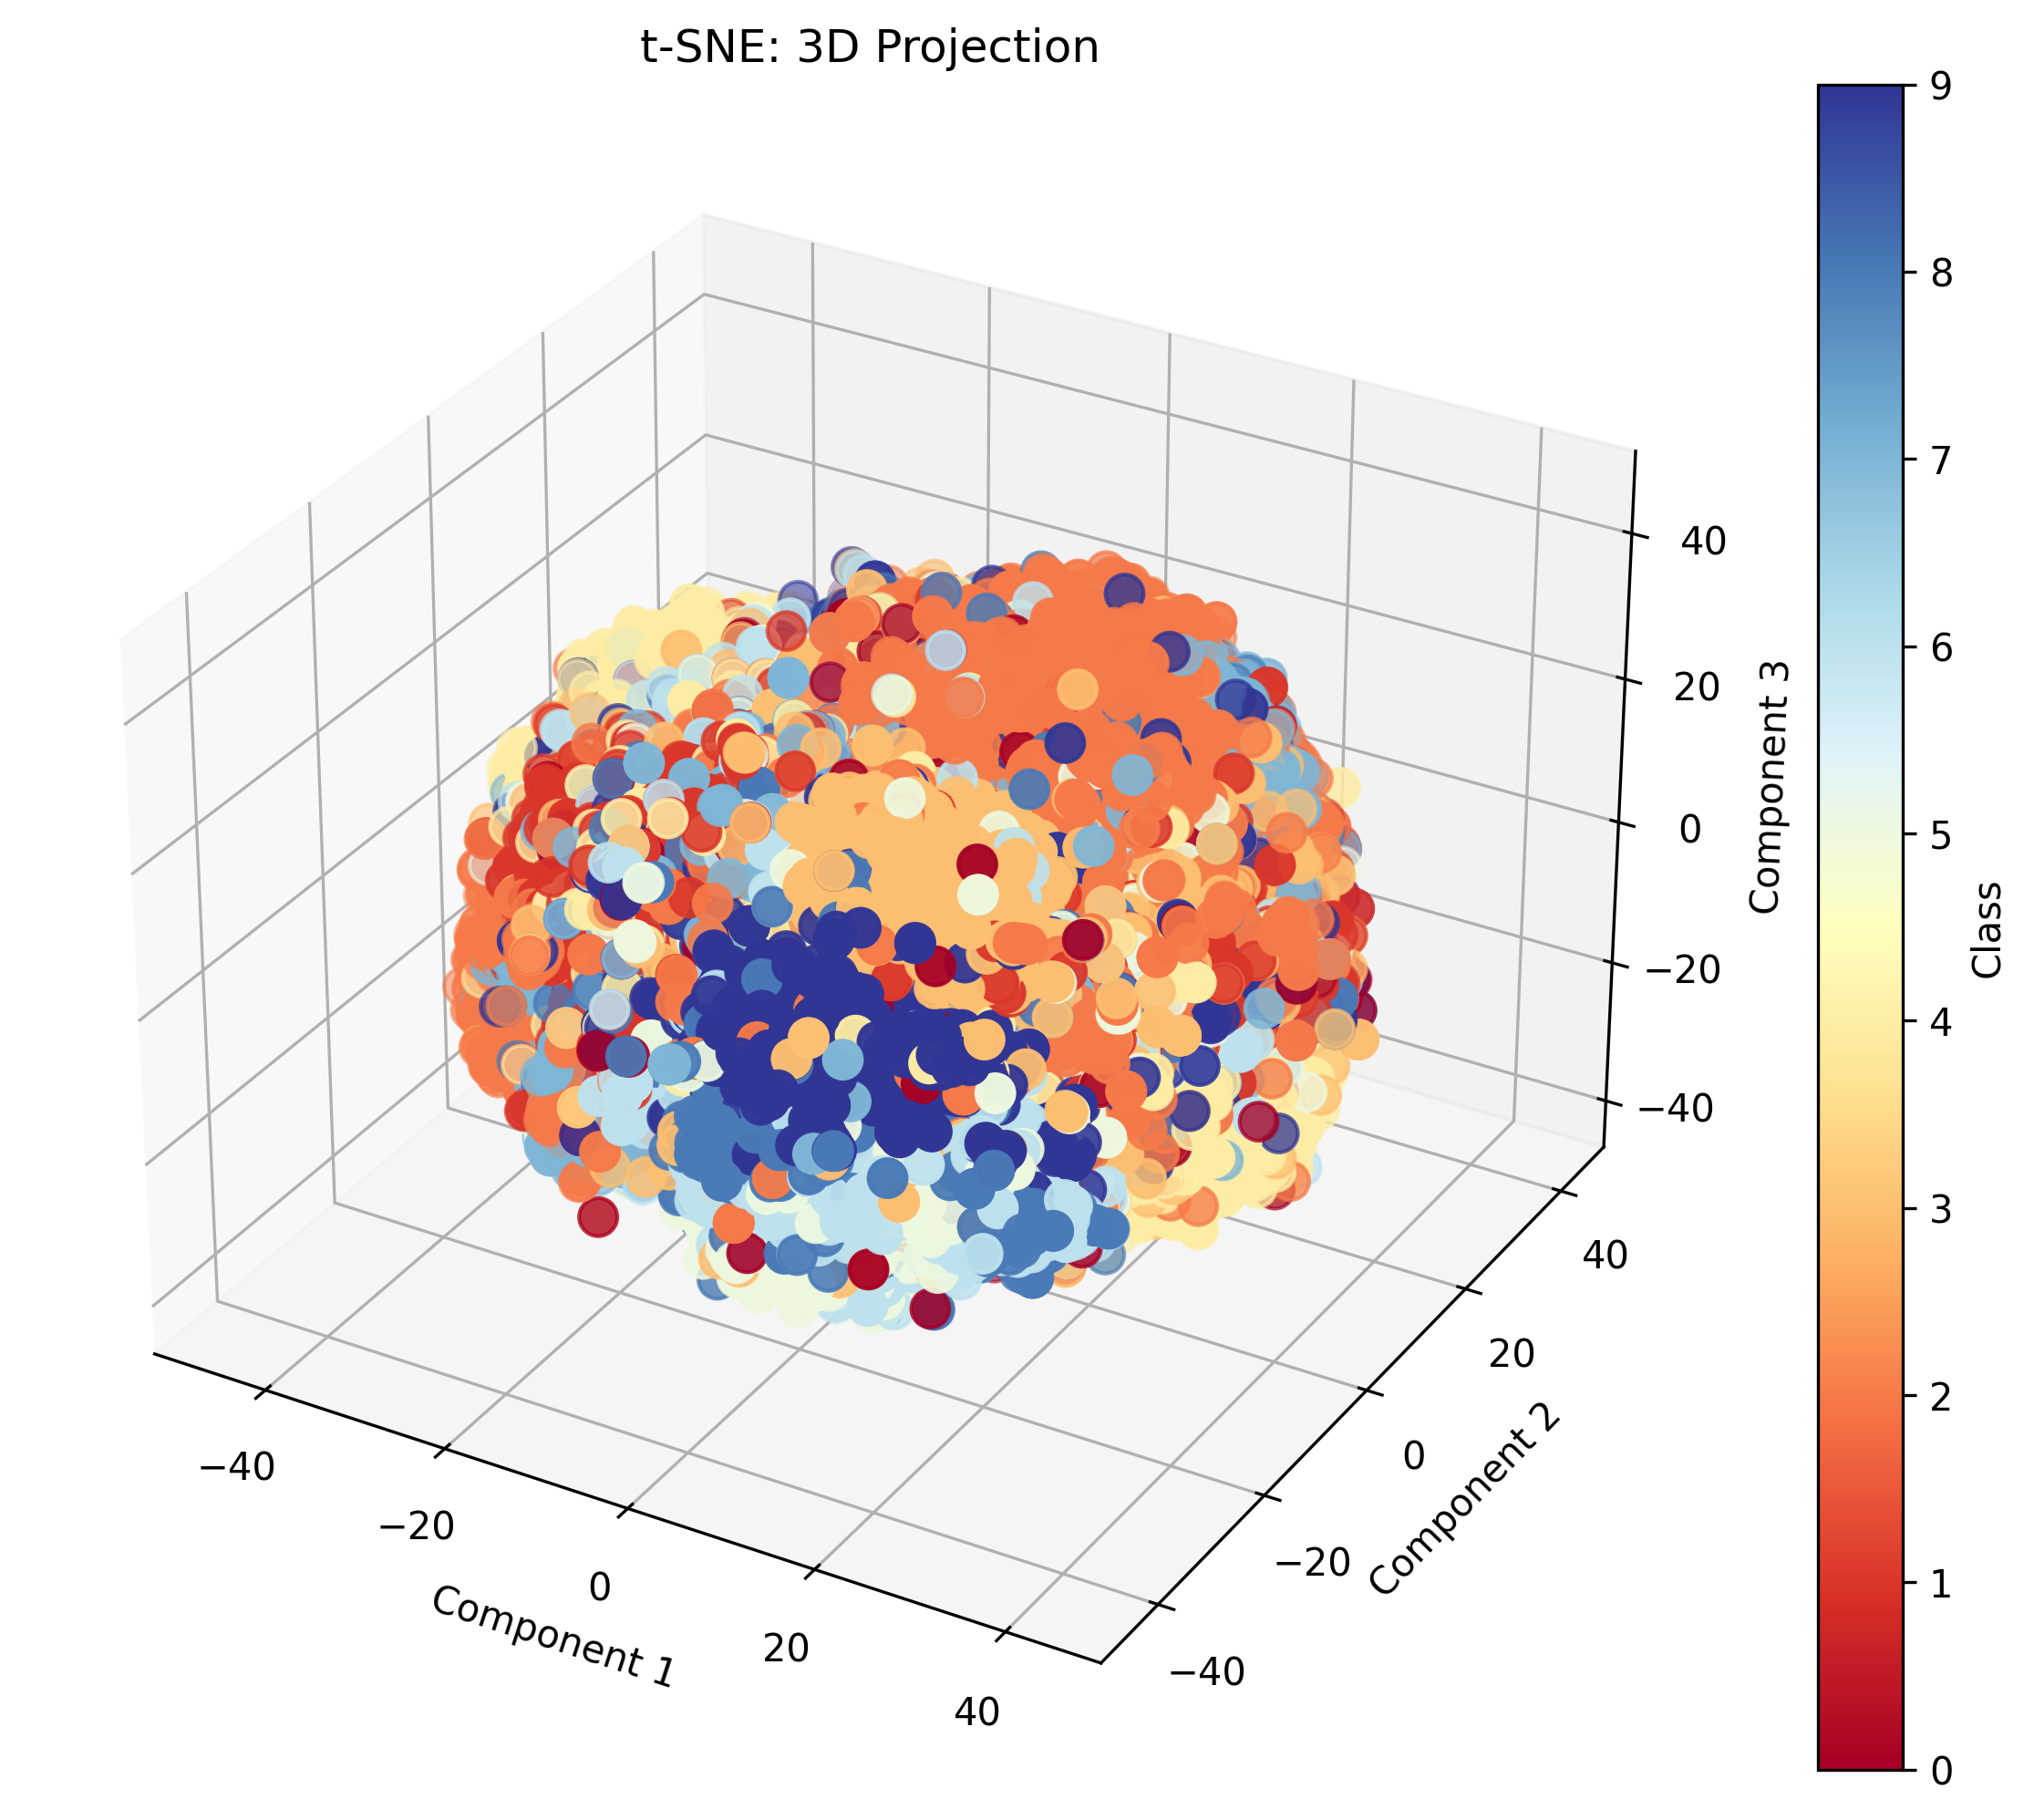
\includegraphics[width=0.9\linewidth]{figures/tsne_3d_projection.png}
        \caption{tSNE: 3D}
        \label{fig:tsne_3d}
\end{figure}

\subsection{Selección de modelos}
Por lo visto en clase, además de los modelos para reducción de dimensiones, se consideran las siguientes opciones para experimentación:
\begin{itemize}
        \item KNeighborsClassifier (KNN)\cite{scikit-learn-knn}
        \item LogisticRegression\cite{scikit-learn-logreg}
        \item Support Vector Machines (SVM)\cite{scikit-learn-svm}
\end{itemize}

Cada modelo fue evaluado con el mismo dataset de entrenamiento para seleccionar aquel que tuviera el mayor score. Se recurrió a un barrido de hiperparámetros para lograr esta tarea. El propósito final es mantener un solo modelo después de comparar los datos y rendimiento de cada uno.

\subsection{Cross-Validation de modelos con CUDA}
Se realizó un GridSearch manual inspirado en la implementación de scikit-learn vista en clase\cite{scikit-learn_gridsearchcv}. En este caso, varios ciclos iterativos anidados exploran diferentes combinaciones de hiperparámetros haciendo fit y score en diferentes pipelines. Se utilizaron módulos de cuML\cite{cuml2023} que son análogos a las implementaciones de scikit-learn con la ventaja de ser acelerados por GPU. En todos los experimentos se utilizó una RTX 3080. Los siguientes rangos y combinaciones fueron probados, la métrica de score se obtuvo con el dataset Test.

\begin{otherlanguage}{english}
\begin{itemize}
        \item PCA y KNN
        \begin{itemize}
                \item PCA components: \( \{ x \in \mathbb{Z} \mid 1 \leq x \leq 60 \} \)
                \begin{itemize}
                        \item Mejor: 55
                \end{itemize}
                \item KNN neighbors: \( \{ x \in \mathbb{Z} \mid 30 \leq x \leq 100 \} \)
                \begin{itemize}
                        \item Mejor: 32
                \end{itemize}
        \end{itemize}

        \item PCA y SVM
        \begin{itemize}
                \item PCA components: \( \{ x \in \mathbb{Z} \mid 1 \leq x \leq 60 \} \)
                \begin{itemize}
                        \item Mejor: 57
                \end{itemize}
                \item SVM regularization \( C \): \( \{ 0.0001, 0.001, 0.01, 0.1, 1 \} \)
                \begin{itemize}
                        \item Mejor: 1
                \end{itemize}
                \item SVM kernel types: \( \{ \text{linear}, \text{rbf}, \text{poly} \} \)
                \begin{itemize}
                        \item Mejor: poly
                \end{itemize}
                \item SVM polynomial degree: \( \{ x \in \mathbb{Z} \mid 2 \leq x \leq 8 \} \)
                \begin{itemize}
                        \item Mejor: 6
                \end{itemize}
        \end{itemize}

        \item PCA y LogisticRegression
        \begin{itemize}
                \item PCA components: \( \{ x \in \mathbb{Z} \mid 55 \leq x \leq 79 \} \)
                \begin{itemize}
                        \item Mejor: 57
                \end{itemize}
                \item Regularization \( C \): \( \{ 0.0001, 0.001, 0.01, 0.1, 1, 10 \} \)
                \begin{itemize}
                        \item Mejor: 0.001
                \end{itemize}
                \item Log max iterations: \( C \): \( \{ 100, 1000, 10000 \} \)
                \begin{itemize}
                        \item Mejor: 100
                \end{itemize}
        \end{itemize}

        \item UMAP y SVM
        \begin{itemize}
                \item UMAP components: \( \{ x \in \mathbb{Z} \mid 30 \leq x \leq 50 \} \)
                \begin{itemize}
                        \item Mejor: 47
                \end{itemize}
                \item UMAP neighbors: \( \{ x \in \mathbb{Z} \mid 5 \leq x \leq 50 \} \)
                \begin{itemize}
                        \item Mejor: 15
                \end{itemize}
                \item UMAP mindist: \( C \): \( \{ 0.001, 0.01, 0.1, 1 \} \)
                \begin{itemize}
                        \item Mejor: 1
                \end{itemize}
                \item UMAP Metric: \( \{ \text{hamming}, \text{manhattan}, \text{cosine}, \allowbreak \text{euclidean} \} \)
                \begin{itemize}
                        \item Mejor: cosine
                \end{itemize}
                \item SVM regularization \( C \): \( \{ 1 \} \)
                \item SVM kernel types: \( \{ \text{poly} \} \)
                \item SVM polynomial degree: \( \{ x \in \mathbb{Z} \mid 4 \leq x \leq 6 \} \)
                \begin{itemize}
                        \item Mejor: 4
                \end{itemize}
        \end{itemize}
        
\end{itemize}
\end{otherlanguage}

Después de evaluar todos los resultados, la combinación de modelos con mejor resultado fue \textbf{PCA y SVM} con score de \textbf{0.80}.

tSNE fue excluido de la búsqueda por falta de recursos computacionales.

\begin{figure}[H]
        \centering
        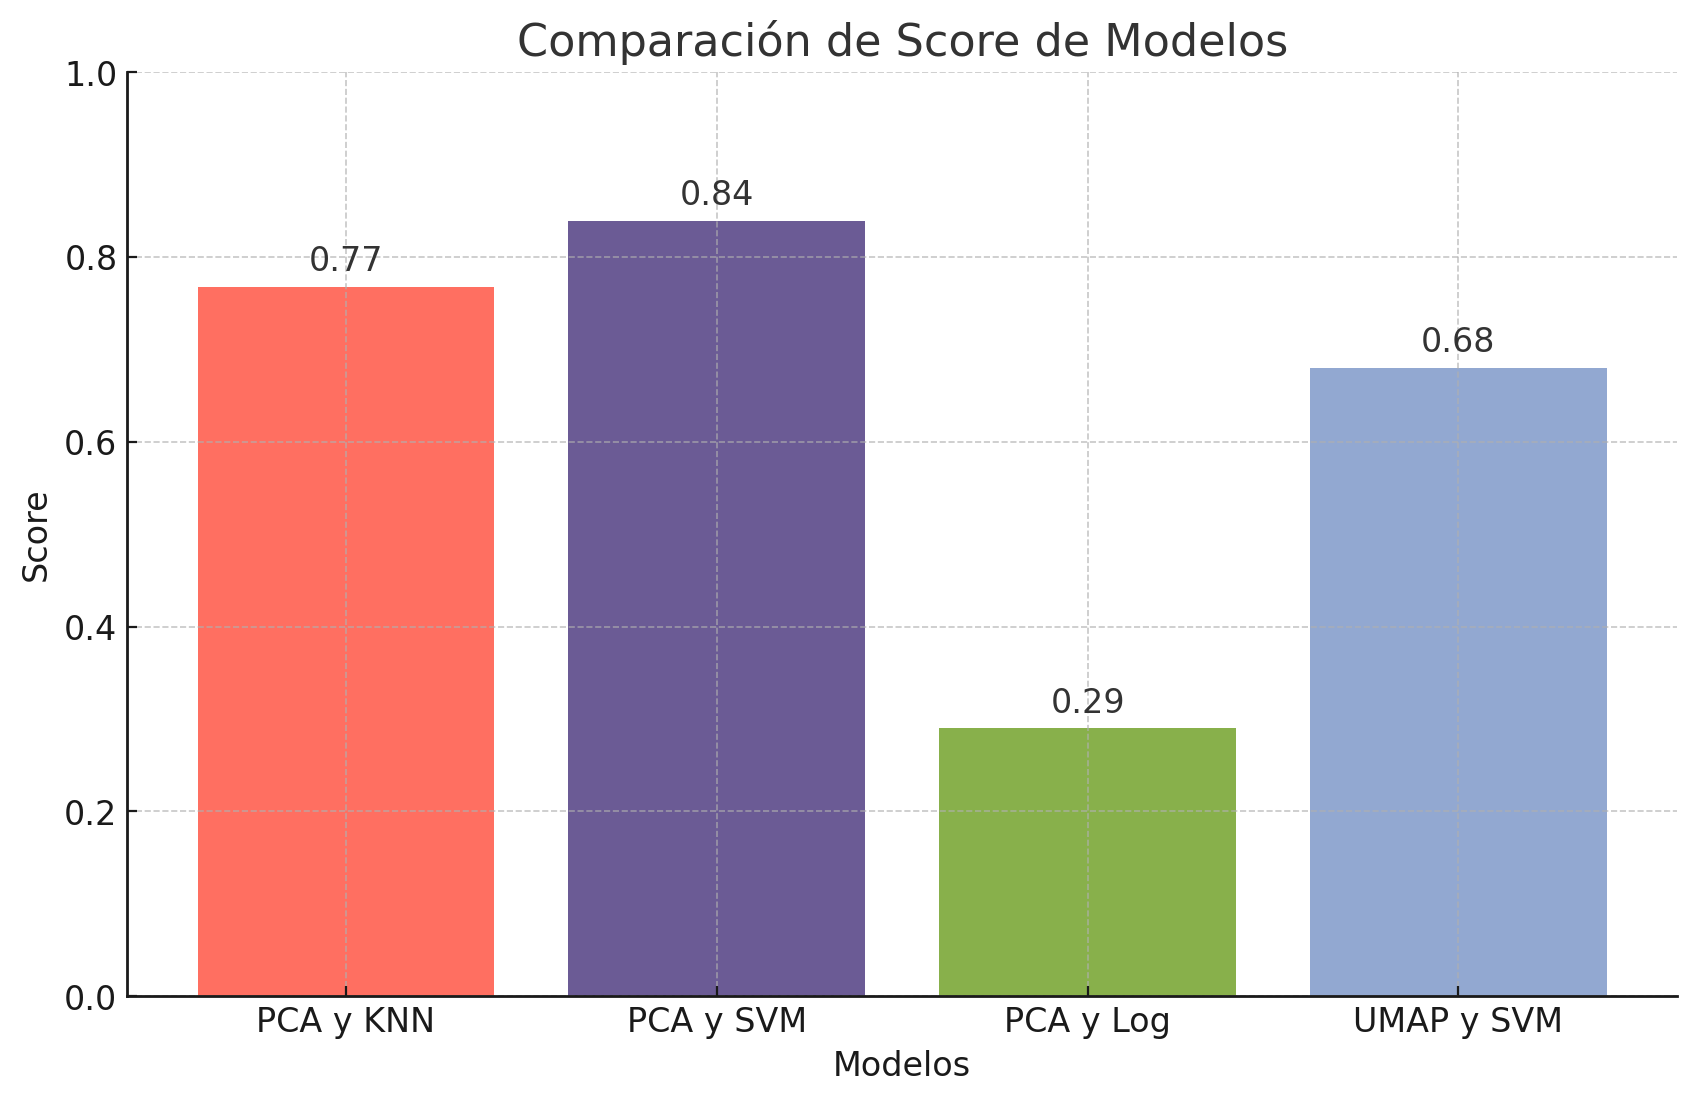
\includegraphics[width=\linewidth]{figures/comparacion_modelos.png}
        \caption{Score de modelos con resultados de Cross-Validation}
        \label{fig:comparativa_modelos}
\end{figure}

\subsection{Cross-Validation de pre-procesamiento}
De forma similar a la sección anterior, se realizó un GridSearch para encontrar los valores óptimos en la etapa de pre-procesamiento. Una vez seleccionada una combinación de modelos e hiperparámetros (PCA y SVM), se probaron las siguientes combinaciones:

\begin{otherlanguage}{english}
        \begin{itemize}
                \item Sólo hacer escala de grises: \( \{ \text{True}, \text{False} \} \)
                \begin{itemize}
                        \item Mejor: False
                \end{itemize}
                \item Aplicar filtro Gaussiano: \( \{ \text{True}, \text{False} \} \)
                \begin{itemize}
                        \item Mejor: True
                \end{itemize}
                \item Sigma Gaussiano: \( \{ x \in \mathbb{Z} \mid 1 \leq x \leq 10 \} \)
                \begin{itemize}
                        \item Mejor: 9
                \end{itemize}
                \item Transformación post-CLAHE: \( \{ \text{median}, \text{log} \} \)
                \begin{itemize}
                        \item Mejor: median
                \end{itemize}
        \end{itemize}
\end{otherlanguage}

\begin{figure}[H]
        \centering
        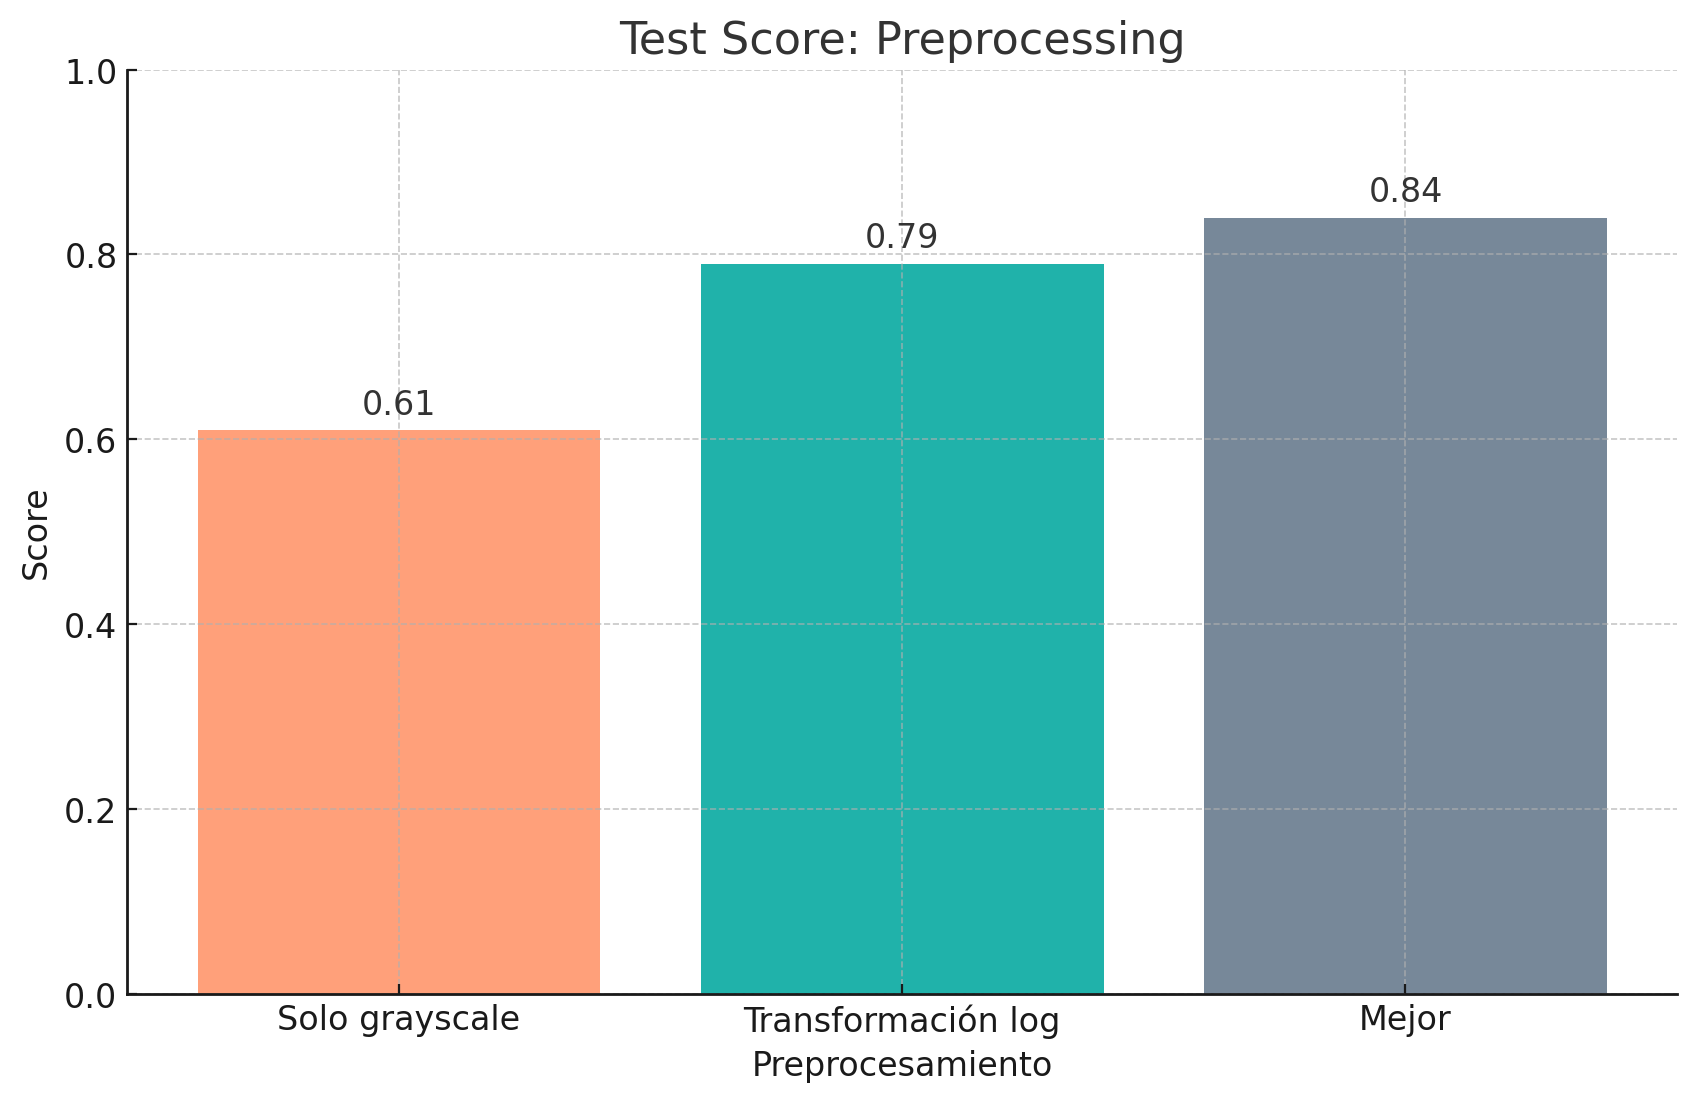
\includegraphics[width=\linewidth]{figures/preprocessin_gridsearch.png}
        \caption{Score de mejor modelo con diferentes parámetros de preprocesamiento}
        \label{fig:comparativa_preprocesamiento}
\end{figure}

\subsection{Entrenamiento y Validación}
Una vez ejecutado el paso de Cross-Validation, se cuenta con un conjunto de hiperparámetros que pueden usarse para entrenar y obtener el score de nuestro modelo con los datos pre-procesados. Para esto, basta con re-utilizar el mismo Pipeline definido en la búsqueda de hiperparámetros utilizando los valores antes encontrados.

\begin{lstlisting}[language=Python]
validation_pipeline = Pipeline(
        steps=[
        ('preprocessing', PreprocessingTransformer(
                gaussian_sigma=9,
                extra_filter='median',
                use_gpu=True)),
        ('pca', cuPCA(
                n_components=57)),
        ('svm', cuSVC(
                C=1,
                kernel='poly',
                degree=6))])

validation_pipeline.fit(X_train, Y_train)

Y_test_predict = validation_pipeline.predict(
                 ds_test_images)
accuracy_score(Y_test, Y_test_predict.get())

Y_train_predict = validation_pipeline.predict(
                  X_train)
accuracy_score(Y_train, Y_train_predict.get())
\end{lstlisting}

\begin{figure}[H]
        \centering
        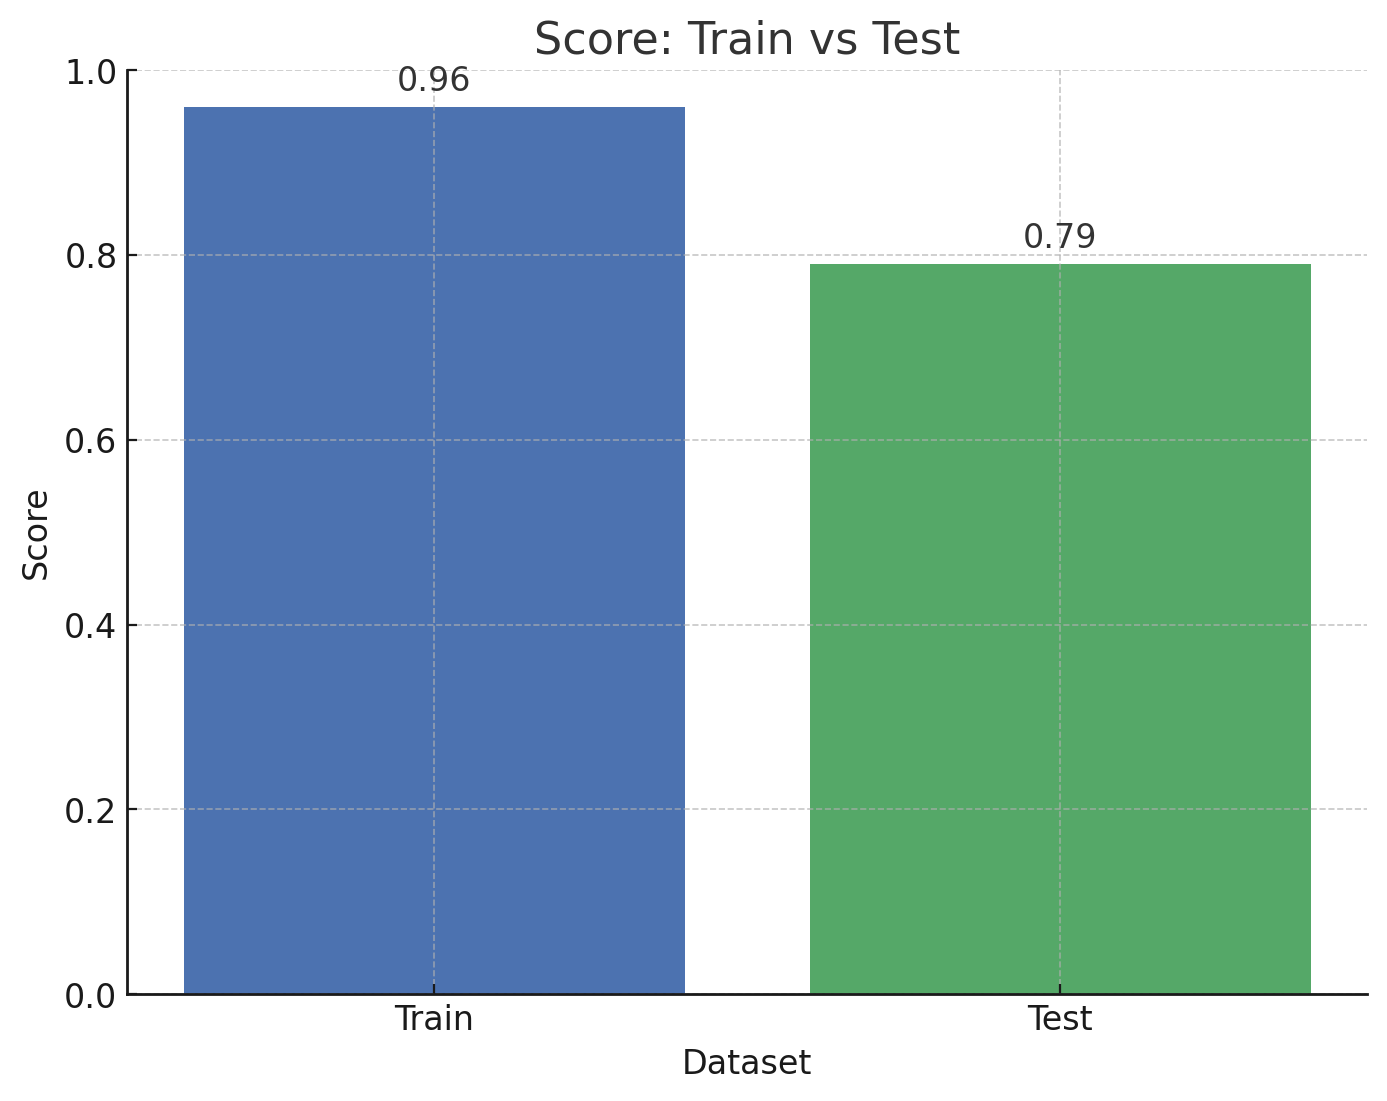
\includegraphics[width=0.9\linewidth]{figures/train_vs_test_final.png}
        \caption{Comparativa de score, modelo final, datasets Train y Test}
        \label{fig:score_train_vs_test}
\end{figure}

\section{Matriz de confusión y balanceo de dataset}
En los experimentos iniciales se logró observar un desbalanceo en el dataset de entrenamiento ya que el dígito 1 tenía significativamente más muestras que los otros dígitos en el dataset. Esto podría implicar un problema en el que no se representan de forma uniforme todas las posibles etiquetas de nuestros datos. La matriz de confusión muestra este comportamiento.

\begin{figure}[H]
        \centering
        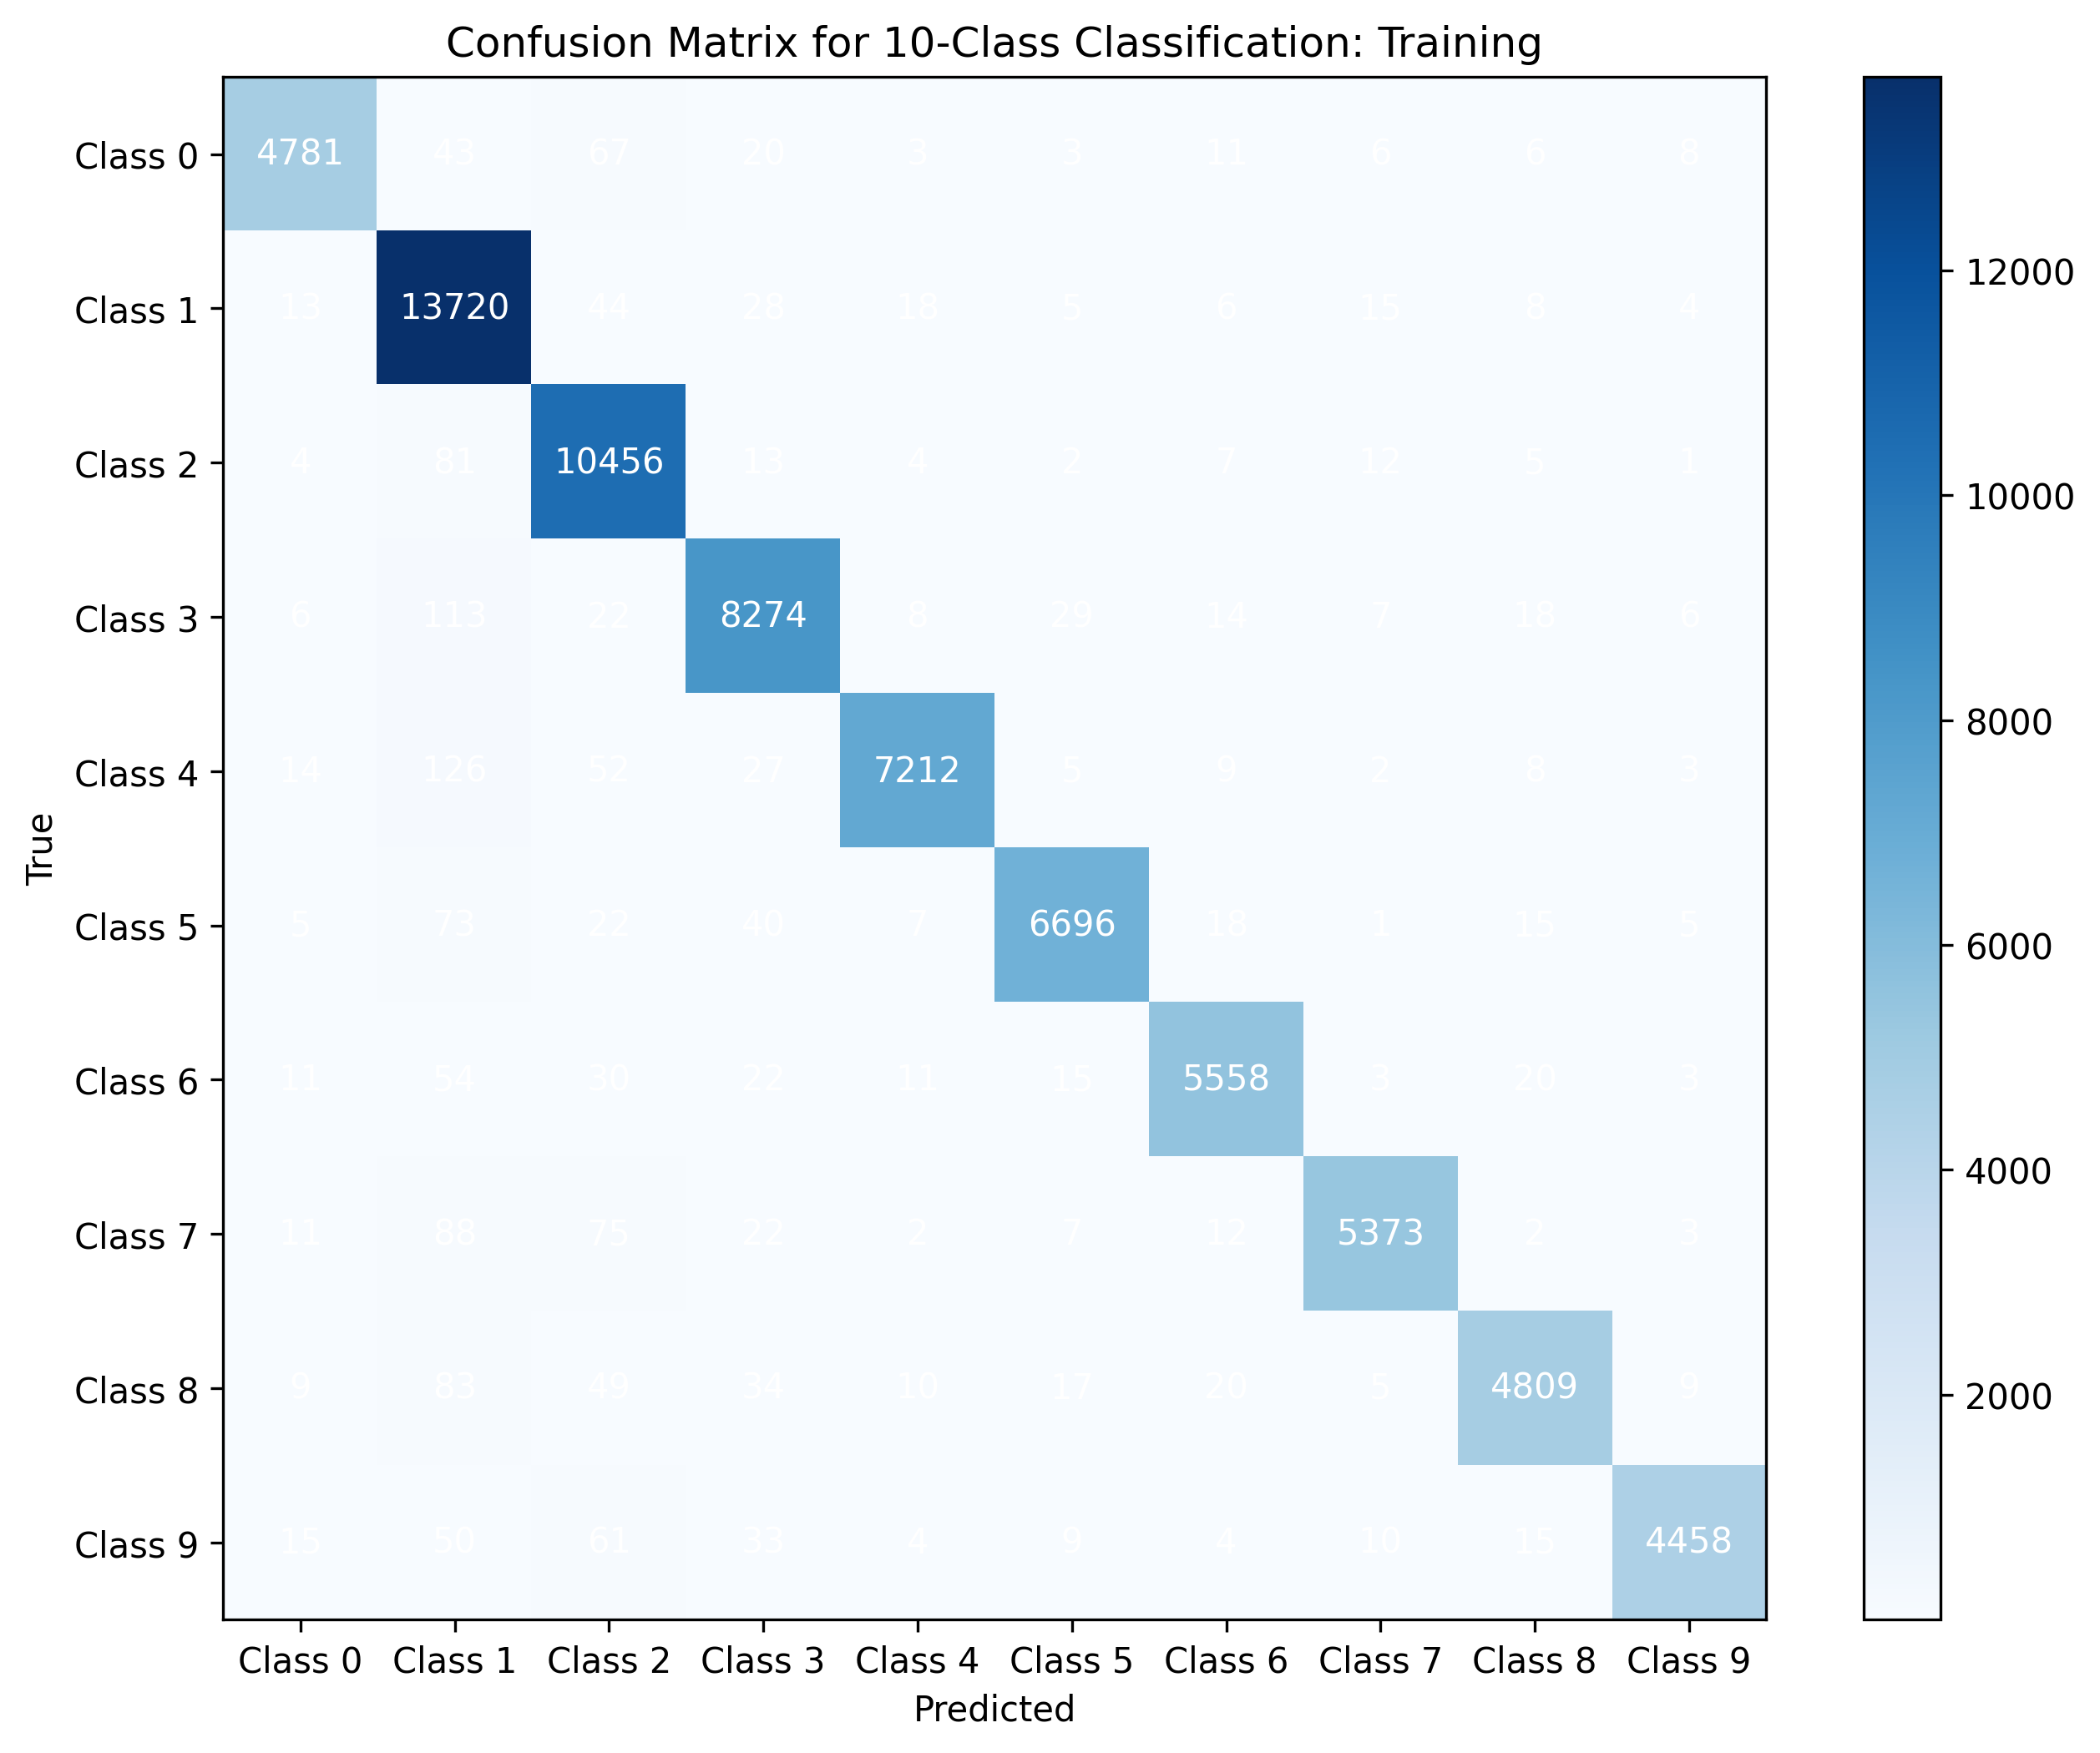
\includegraphics[width=\linewidth]{figures/confusion_matrix_Training_preSMOTE.png}
        \caption{Matriz de confusión, Train dataset, desbalance por dígito 1}
        \label{fig:confusion_matrix_pre_smote}
\end{figure}

Se utilió SMOTE\cite{smote2023} para balancear el dataset. La tarea de Cross-Valiation se hizo con el dataset de training original, la validación se realizó con SMOTE. Sólo logró observarse una ligera degradación en el score de aproximadamente \textbf{1\%}. Una vez aplicado este aumento de datos, se observa una matriz de confusión balanceada.

\begin{figure}[H]
        \centering
        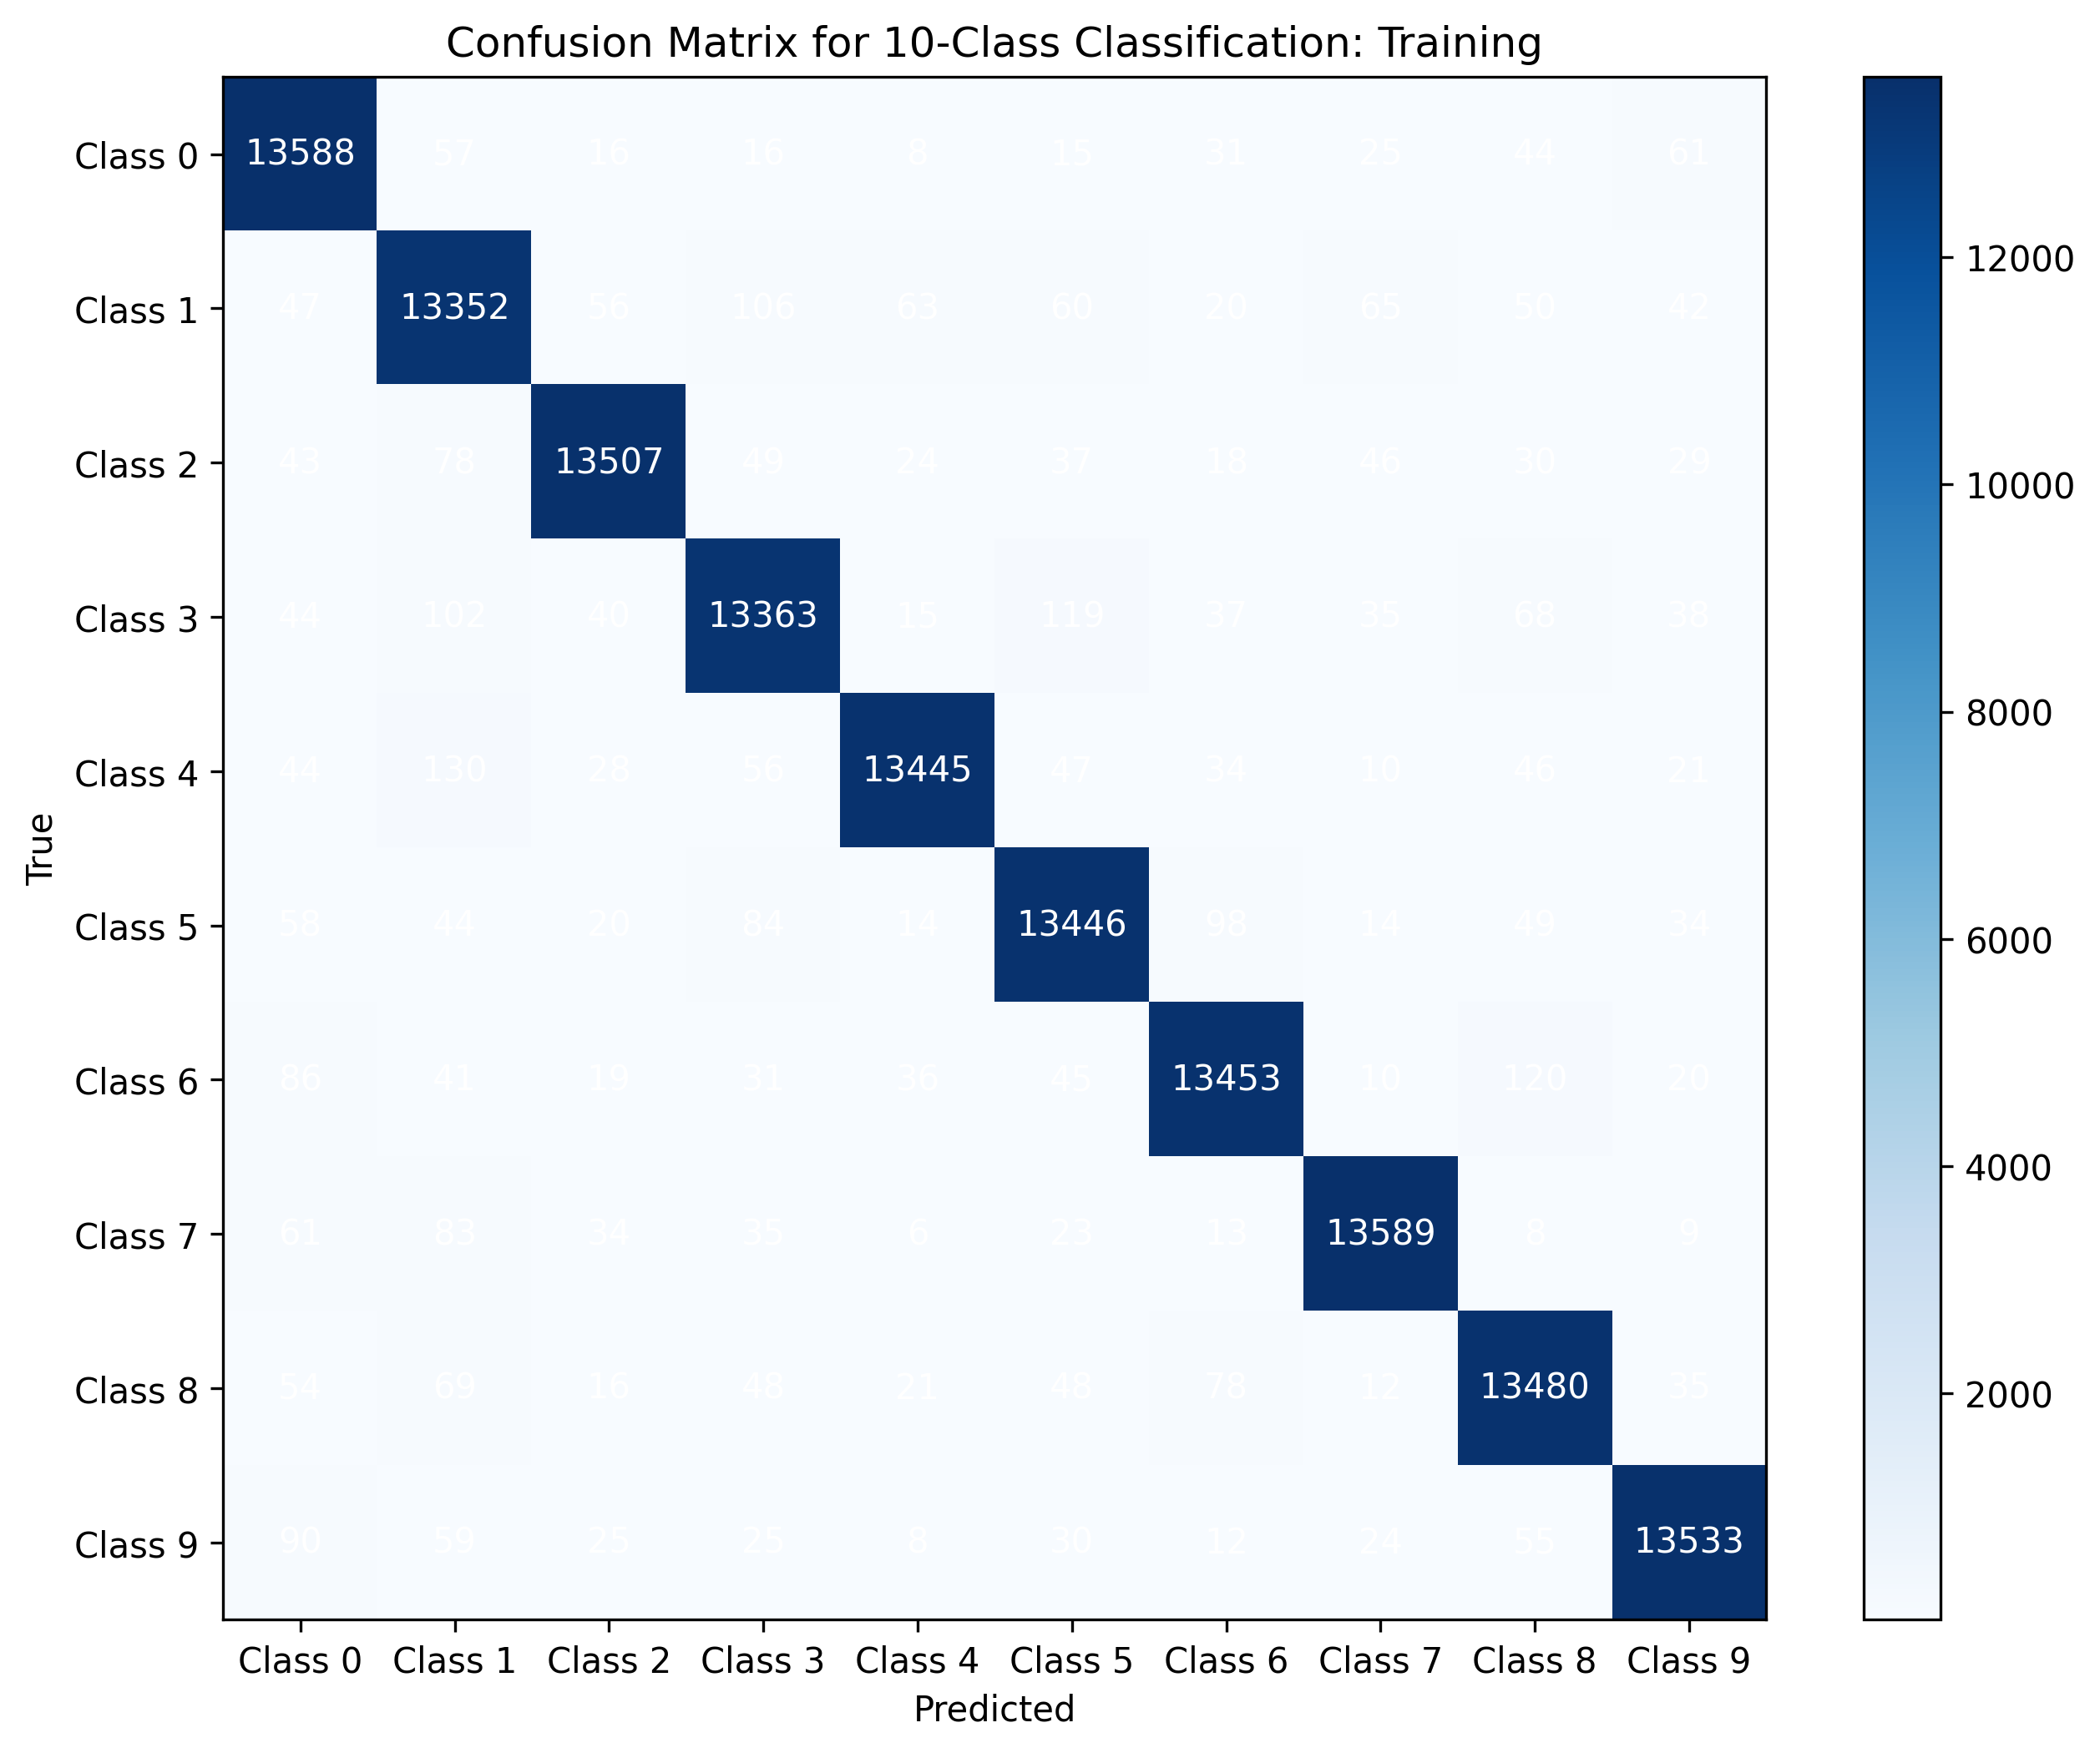
\includegraphics[width=\linewidth]{figures/confusion_matrix_Training_wSMOTE.png}
        \caption{Matriz de confusión, Train dataset con SMOTE}
        \label{fig:confusion_matrix_post_smote}
\end{figure}

El dataset Test muestra el mismo comportamiento, sin embargo no se aplicó SMOTE a este dataset ya que es usado para validación, no para entrenamiento.

\begin{figure}[H]
        \centering
        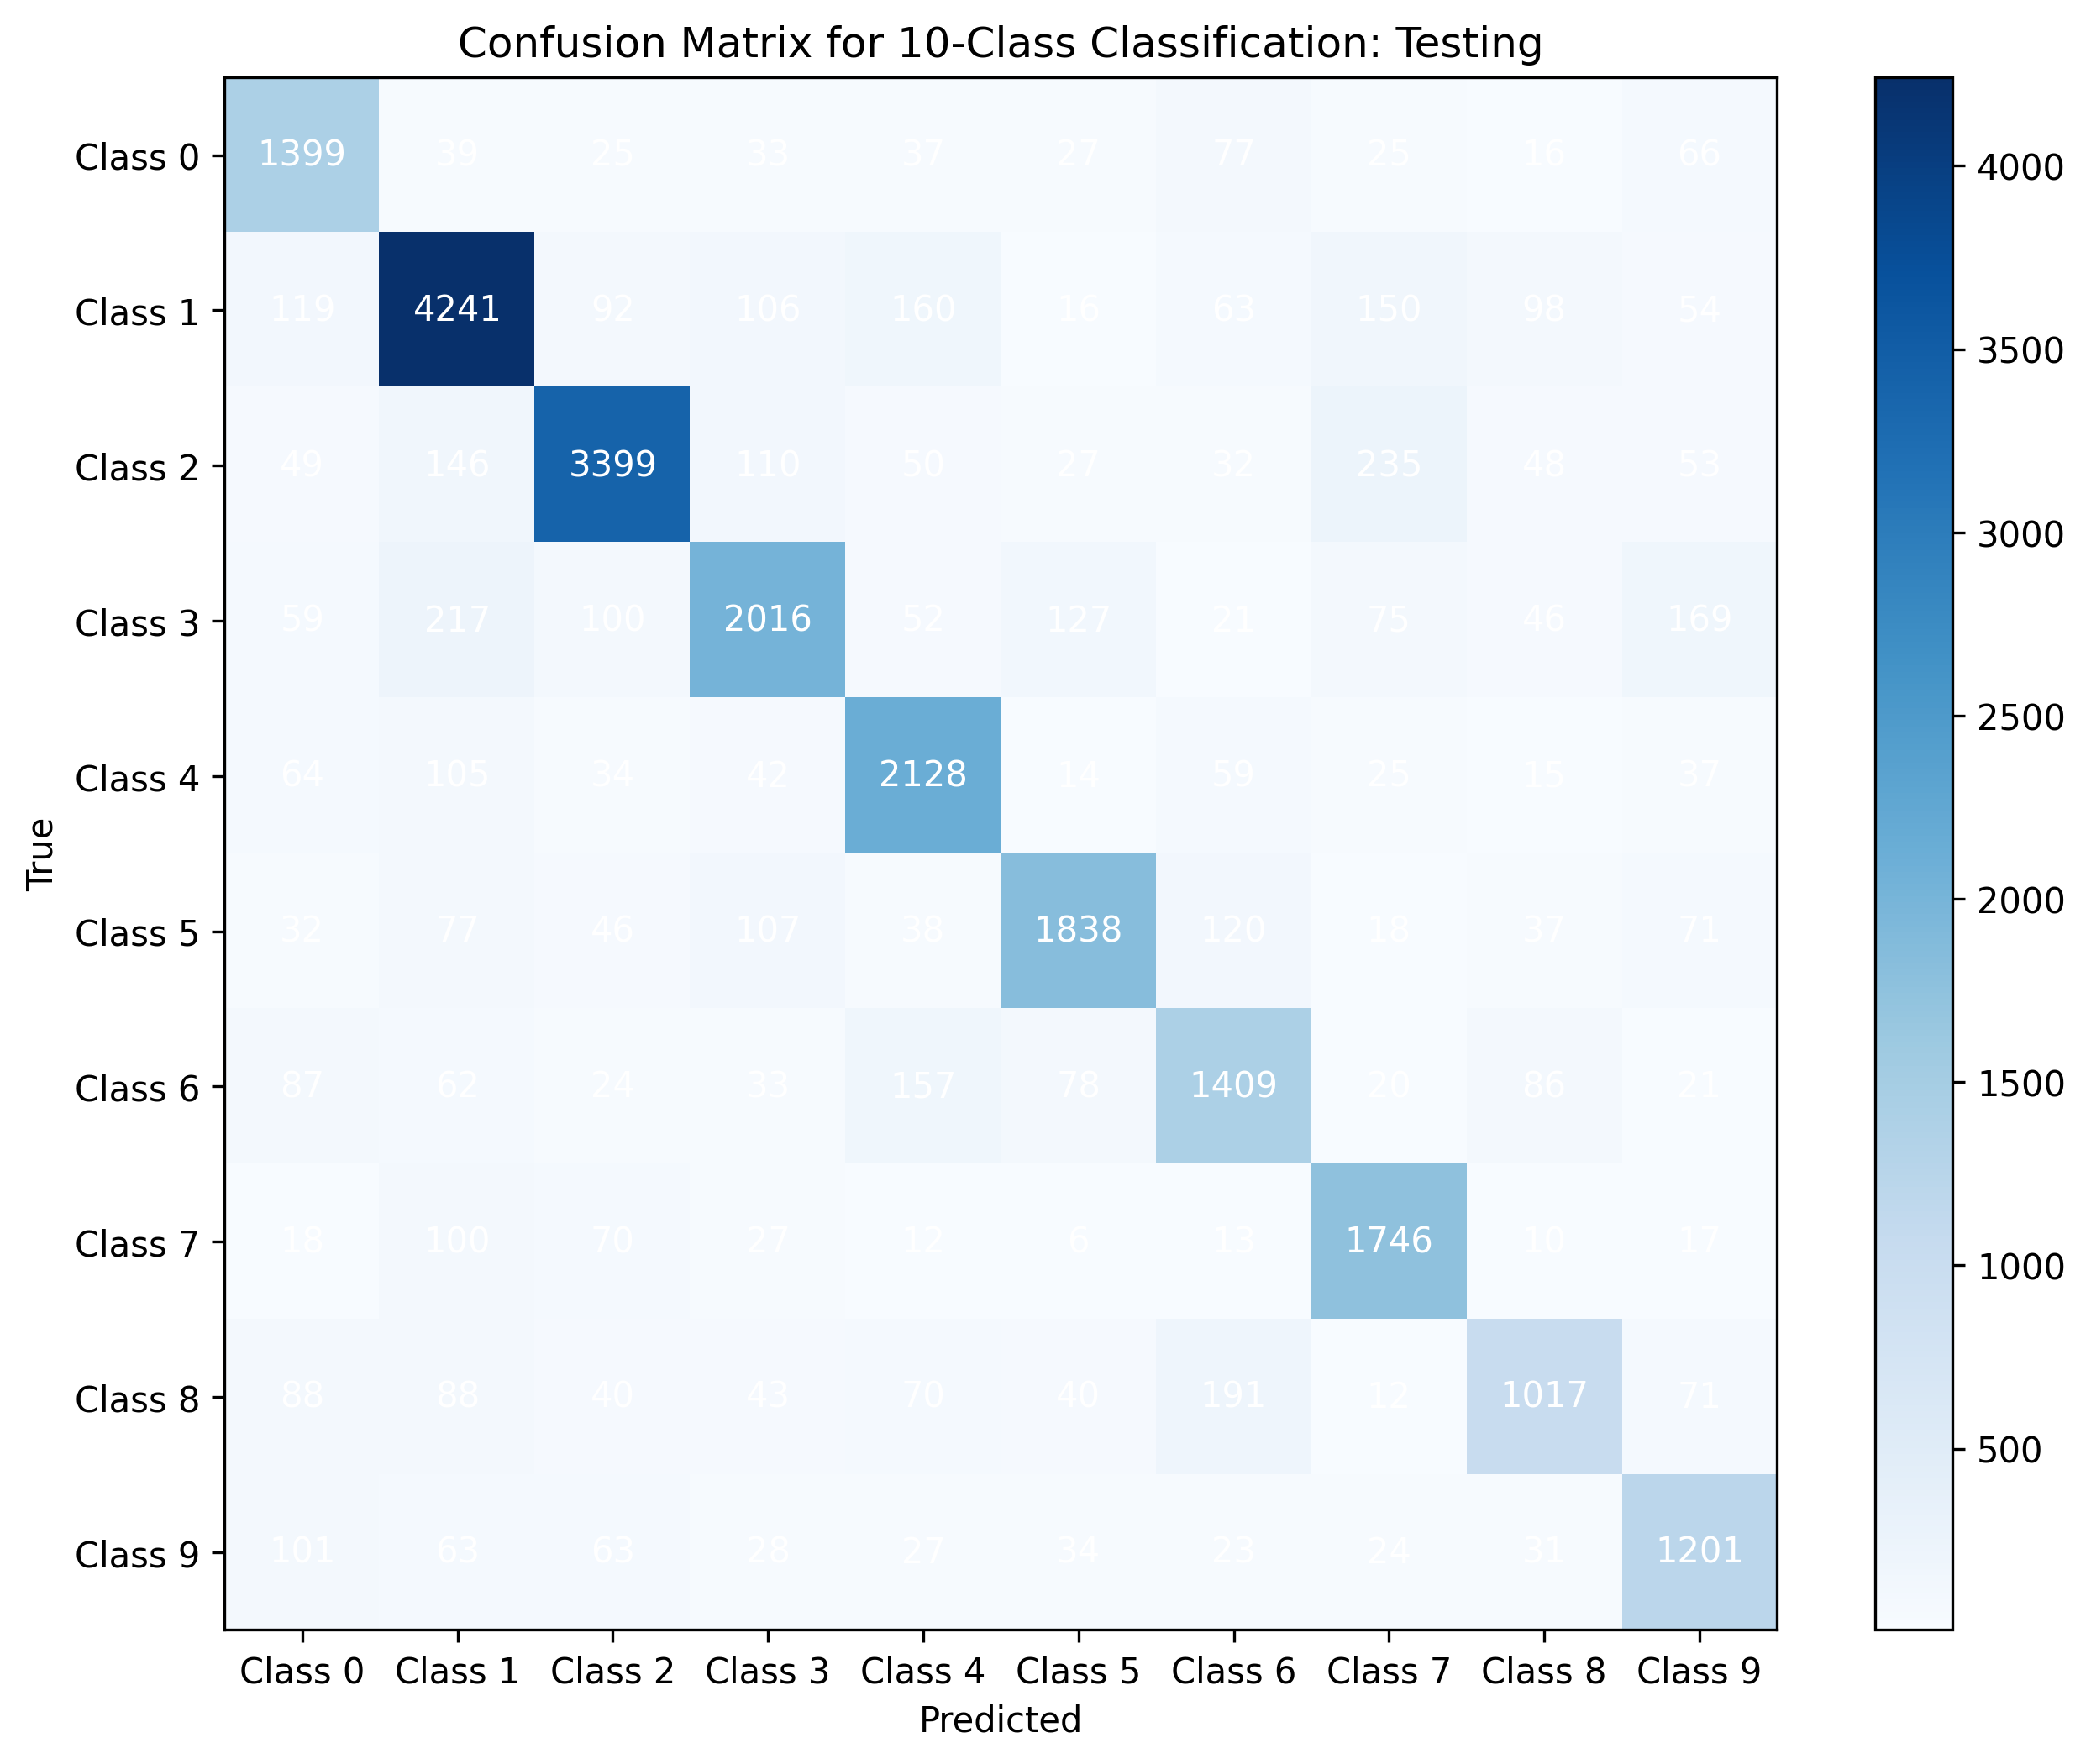
\includegraphics[width=\linewidth]{figures/confusion_matrix_Testing_wSMOTE.png}
        \caption{Matriz de confusión, Test dataset}
        \label{fig:confusion_matrix_test}
\end{figure}

\section{Conclusiones}

\subsection{Preprocesamiento y Feature Engineering}
Se propone una serie de pasos para transformar de distintas formas cada muestra del dataset. Visualmente y en varios ejemplos se observa cómo cada proceso modifica la información y podría permitir una extracción o representación más concisa del objetivo final. En los esfuerzos iniciales se consideró detección de contornos, pero esta transformación fue descartada porque impactaba negativamente el rendimiento. Se demuestra también el impacto de estos pasos de preprocesamiento, ya que el score con una simple conversión a escala de grises tiene un valor bajo (0.57 vs 0.79).

\subsection{Reducción de dimensionalidad}
Siguiendo el ejemplo con datasets como MNIST, se experimentó con modelos no supervisados que ayudan a reducir las dimensiones (PCA, UMAP, tSNE). A pesar de ser un problema similar para reconocimieno de dígitos, el dataset SVHN representa complicaciones por su variedad de colores, dígitos o elementos distractores además de inconsistencia entre el color o luminosidad de el fondo y dígito.

Las gráficas 2D y 3D en los diferentes modelos muestran dificultad para observar grupos bien definidos y separados, lo que sugiere que este problema necesita más dimensiones que las observables. Una vez se realizó CrossValidation es posible confirmar que el número de componentes con mejor redimiento es bastante alejado a las dimensiones que se pueden observar fácilmente, el hiperparámetro componentes PCA tuvo un valor final de 57.

\subsection{Selección de modelos y Cross-Validation}
La aceleración con CUDA resultó crucial para este proceso, ya que las iteraciones utilizando CPU eran significativamente más lentas. Esto permitió explorar varios modelos y un rango más amplio de hiperparámetros.

En todos los casos se observa claramente que se obtiene un mejor rendimiento con un número significativo de dimensiones. Esto sugiere que el dataset es complejo y necesita mucho más dimensiones que las observables a simple vista para poder representarse correctamente. A pesar de visualmente mostrar mejor separación en las gráficas 2D y 3D, UMAP no resultó ser el modelo con mejor rendimiento.

La ventaja de PCA en este caso puede sugerir que existe una relación lineal entre los valores de las múltiples dimensiones y la etiqueta de cada muestra. 

Los rangos limitados de exploración se deben a una falta de recursos computacionales, se encontraron problemas con UMAP en dimensiones muy altas y tSNE en particular.

\subsection{Entrenamiento y Validación}
Se logra observar un score aceptable, \textbf{0.96} en training y \textbf{0.79} en testing. Esto sugiere que el modelo no está realizando overfitting total ni simplemente memorizando el dataset de entrenamiento, por lo que logra generalizar la relación entre los valores de los pixeles en la imagen y el dígito que se encuentra en el centro. Se reconoce que existen modelos más adecuados para reconocimiento de imagen con mucho mejor rendimiento, por ejemplo, redes neuronales. Sin embargo, estos modelos se encuentran fuera del enfoque de la clase, ya que se consideran de aprendizaje profundo.

\subsection{Matriz de confusión y balanceo de dataset}
Con los resultados iniciales de CrossValidation se logró observar un desbalanceo en el dataset de entrenamiento, específicamente en el dígito 1. Inicialmente se contaban con scores de \textbf{0.97} y \textbf{0.80} en training y testing respectivamente.

Se aplicó SMOTE al dataset de entrenamiento para balancear el número de muestras y la distribución en las diferentes etiquetas, esto para buscar entrenar el modelo con un dataset más representativo y que sea capaz de generalizar para múltiples etiquetas, no solo la que se encuentre más representada.

Los valores de score después de SMOTE bajaron a \textbf{0.96} y \textbf{0.79} en training y testing respectivamente. Esto indica un muy ligero impacto que aún mantiene valores aceptables, indicando que el modelo, con el preprocesamiento e hiperparámetros elegidos, es capaz de generalizar las relaciones entre los pixeles y el dígito encontrado al centro de la imagen.

% if have a single appendix:
%\appendix[Proof of the Zonklar Equations]
% or
%\appendix  % for no appendix heading
% do not use \section anymore after \appendix, only \section*
% is possibly needed

% use appendices with more than one appendix
% then use \section to start each appendix
% you must declare a \section before using any
% \subsection or using \label (\appendices by itself
% starts a section numbered zero.)
%


\printbibliography
\end{document}


